%------------------ vorlage.tex ------------------------------------------------
%
% LaTeX-Vorlage zur Erstellung von Projektdokumentationen
% im Fachbereich Informatik der Hochschule Trier
%
% Basis: Vorlage 'svmono' des Springer Verlags
% Bearbeiter: Hermann Schloß, Christian Bettinger
%
%-------------------------------------------------------------------------------


%------------------ Präambel ---------------------------------------------------
\documentclass[envcountsame, envcountchap, deutsch]{i-studis}

\usepackage[utf8]{inputenc}

\usepackage[a4paper]{geometry}
\usepackage[english, ngerman]{babel}

\usepackage[pdftex]{graphicx}
\usepackage{epstopdf}

\usepackage{listings}
\usepackage{titlesec}
\setcounter{secnumdepth}{4}

\usepackage[german, ruled, vlined]{algorithm2e}
\usepackage{amssymb, amsfonts, amstext, amsmath}
\usepackage{array}
\usepackage[skip=10pt]{caption}
\usepackage[usenames, dvipsnames]{color}
\usepackage[pdftex, plainpages=false]{hyperref}
\usepackage{textcomp}

\usepackage{bibgerm}
\bibliographystyle{geralpha}

\usepackage{xcolor} % Include the xcolor package for color definitions
\definecolor{lightgray}{gray}{0.9} % Define the lightgray color

\usepackage{graphicx}
\usepackage{placeins} % For \FloatBarrier
\usepackage{float} % Include this package for the [H] option



\usepackage{makeidx}
\usepackage{multicol}
\makeindex

\pagestyle{myheadings}
\setlength{\textheight}{1.1\textheight}

\lstset{
	basicstyle=\scriptsize\ttfamily,
	commentstyle=\scriptsize\ttfamily\color{Gray},
	identifierstyle=\scriptsize\ttfamily,
	keywordstyle=\scriptsize\ttfamily,
	stringstyle=\scriptsize\ttfamily,
	tabsize=4,
	numbers=left,
	numberstyle=\tiny,
	numberblanklines=false,
	frame=single,
	framesep=3mm,
	framexleftmargin=7mm,
	xleftmargin=10mm,
	linewidth=144mm,
	captionpos=b,
}


%------------------ Manuelle Silbentrennung ------------------------------------
\hyphenation{Ele-men-tar-ob-jek-te ab-ge-tas-tet Aus-wer-tung House-holder-Matrix Least-Squares-Al-go-ri-th-men}


%------------------ Titelseite -------------------------------------------------
\begin{document}

\title{ShopNook: E-Commerce Warenkorbanwendung mit Spring Boot}
\subtitle{ShopNook: Development of an e-commerce shopping cart application with Spring Boot}

\author{Imad-Eddine Abdessami, Mohammed Salih Mezraoui}

\supervisor{Prof. Dr. Andreas Lux}

\address{Trier}
\submitdate{den 29.08.2024}

%------------------ Projektart -------------------------------------------------
\project{Bachelor-Projektarbeit}
%\project{Bachelor-Abschlussarbeit}
%\project{Master-Projektstudium}
%\project{Master-Abschlussarbeit}
%\project{Seminar}
%\project{Hausarbeit}

\mytitlepage

%------------------ Vorwort, Kurzfassung, Verzeichnisse ------------------------
\frontmatter
%\preface

Ein Vorwort ist nicht unbedingt nötig. Falls Sie ein Vorwort schreiben, so ist dies der Platz, um z.B. die Firma vorzustellen, in der diese Arbeit entstanden ist, oder um den Personen zu danken, die in irgendeiner Form positiv zur Entstehung dieser Arbeit beigetragen haben.

Auf keinen Fall sollten Sie im Vorwort die Aufgabenstellung näher erläutern oder vertieft auf technische Sachverhalte eingehen.
								% Vorwort (optional)
\kurzfassung

Die Arbeit befasst sich mit der Entwicklung einer E-Commerce Warenkorbanwendung, die mit Spring Boot entwickelt wurde. \\
Ziel des Projekts ist es, einen benutzerfreundlichen Online-Marktplatz zu schaffen, der es Kunden ermöglicht, Produkte zu suchen, Artikel in den Warenkorb zu legen und sichere Zahlungen durchzuführen. Die Anwendung integriert Front-End-Technologien wie Angular mit Back-End-Lösungen in Spring Boot und nutzt eine MySQL-Datenbank zur Verwaltung von Benutzer-, Produkt- und Bestelldaten. Besondere Schwerpunkte liegen auf der sicheren Zahlungsabwicklung über die Stripe-API, der HTTPS-Verschlüsselung und der JWT-basierten Authentifizierung, um ein zuverlässiges und sicheres Einkaufserlebnis zu gewährleisten. \\
Diese Arbeit liefert wertvolle Einblicke in die Herausforderungen und Lösungen bei der Entwicklung effizienter Online Shopping-Anwendungen.

							% Kurzfassung/Abstract
\tableofcontents										% Inhaltsverzeichnis
\listoffigures											% Abbildungsverzeichnis (optional)
%\listoftables											% Tabellenverzeichnis (optional)
%\lstlistoflistings										% Listings (optional)


%------------------ Kapitel ----------------------------------------------------
\mainmatter
\chapter{Einleitung und Problemstellung}


Hier werden folgende Aspekte berücksichtigt: 


\begin{itemize}
	\item Ein kleiner Überblick über die Anwendung ShopNook
	\item und deren funktionale, nicht funktionale und technische Anforderungen.
\end{itemize}

\section{Überblick}\index{Überblick}

ShopNook ist ein internetbasierter Marktplatz, der ein nahtloses und angenehmes Einkaufserlebnis bieten soll. Käufer können ganz einfach eine breite Palette von Produkten erkunden, sie in den Warenkorb legen und ihre Einkäufe sicher abschließen. Die Plattform verfügt über ein attraktives und reaktionsfähiges Design, das eine konsistente und ansprechende Benutzererfahrung auf allen Gerätegrößen gewährleistet.\\
Neben der benutzerfreundlichen Oberfläche verfügt ShopNook über robuste Funktionen wie ein Bestandsverwaltungssystem, Benutzerkonten mit verschiedenen Berechtigungen und erweiterte Suchoptionen, die den Käufern helfen, genau das zu finden, was sie brauchen. Die Anwendung ist in der Lage, verschiedene administrative Aufgaben zu erledigen und bietet Käufern einen sicheren und effizienten Checkout-Prozess.

\section{Globale Anforderungen}\index{Globale Anforderungen}

\subsection{Funktionale Anforderungen}

Die App wird über alle notwendigen Funktionen verfügen, um ein reibungsloses Einkaufserlebnis zu gewährleisten. Die Kunden werden die Möglichkeit haben, sich sicher zu registrieren, einzuloggen und einen Produktkatalog zu erkunden. Zu jedem Produkt werden vollständige Details wie Name, Beschreibung, Preis und Bilder angezeigt. Die Kunden können schnell Artikel in ihren Einkaufskorb legen, den Inhalt ändern und zur Zahlung übergehen. Sichere Kreditkartenzahlungen werden während des Kaufvorgangs über die Stripe-API abgewickelt. Administratoren können die Waren überwachen und die Bestellungen im Auge behalten, um sicherzustellen, dass das Online-Geschäft gut funktioniert. 

\subsection{Nich -funktionale Anforderungen}

Die App wird effizient mit gleichzeitigen Nutzern umgehen und die Ladezeiten der Seite sind minimal. HTTPS-Verschlüsselung und JWT-basierte Authentifizierung stellen die Sicherheit in den Vordergrund. Die Einheitlichkeit der Geräte wird durch eine reaktionsschnelle und einfach zu bedienende Schnittstelle gewährleistet.

\subsection{Technische  Anforderungen}

Die vollwertige E-Commerce-App wird mit npm für JavaScript-Dependenzen und Maven für die Java Dependenzen und Build-Prozesse entwickelt. Im Frontend wird Angular verwendet, um eine dynamische und reaktionsschnelle Schnittstelle für die Benutzer bereitzustellen, während im Backend das Spring Boot-Framework verwendet wird, um RESTful APIs zu erstellen. MySQL wird die Datenbank sein, die Benutzer-, Produkt- und Bestelldaten speichert. Git und GitHub werden für die Versionskontrolle verwendet, um Änderungen zu verwalten und die Teamarbeit zu erleichtern. 
\chapter{Methodologie und Systementwurf }

Hier werden über folgende Punkte diskutiert:

\begin{itemize}
	\item Die Entwicklungskonzeption, die wir während der Implementation der Anwendung benutzt haben, sowie die Tools, Technologien und Methodologien. 
	\item Überblick über Spring Boot und seine wichtigste  Funktionalitäten, die auch in dem Projekt angewendet sein werden. 
	\item Detaillierte Erklärung der Struktur und Design der Anwendung (Bsp: Anlyse-/Entwurfsdiagram) 
	\item Datenbanken, UI-Design und unterschiedliche Komponenten des Systems. 
	\item Wie Spring Boot die Entwicklung und Implementation der verschiedenen Module vereinfacht. 
\end{itemize}


\section{Entwurf und Konzeption}\index{Entwurf und Konzeption}

In der Softwareentwicklung spielen Entwurf und Konzeption eine entscheidende Rolle. Diese Phase des Entwicklungsprozesses befasst sich mit der Strukturierung und Planung von Systemen, bevor die eigentliche Implementierung beginnt. 

Ziel ist es, ein klares und verständliches Modell zu erstellen, das die Anforderungen und Funktionen eines Systems abbildet. In diesem Kapitel werden UML und einige Diagrammtypen vorgestellt.

\subsection{UML}\index{UML}

Die Unified Modeling Language (UML) ist ein wesentliches Werkzeug im Bereich Entwurf. UML ist eine standardisierte Modellierungssprache, die eine Vielzahl von Diagrammen bietet, um unterschiedliche Aspekte eines Systems darzustellen. Diese Diagramme helfen dabei, komplexe Systeme zu visualisieren, zu dokumentieren und zu kommunizieren \cite{UML:2023}. 

\subsection{Klassendiagramm}\index{Klassendiagramm}

In diesem Abschnitt stellen wir das Klassendiagramm für die Anwendung vor. Das Diagramm (siehe \ref{fig:class_diagram}) veranschaulicht die wichtigsten beteiligten Klassen, ihre Attribute und die Beziehungen zwischen ihnen.
Das Klassendiagramm dient der Darstellung der Struktur des eCommerce-Systems. Es umfasst die folgenden Klassen:

\begin{itemize}
	\item \textbf{Customer}
	\item \textbf{Order}
	\item \textbf{OrderItem}
	\item \textbf{Address}
	\item \textbf{ProductCategory}
	\item \textbf{Product}
	\item \textbf{State}
	\item \textbf{Country}
\end{itemize}

Die Beziehungen zwischen diesen Klassen sind wie folgt:

\begin{itemize}
	\item Ein \textbf{Kunde} kann mehrere \textbf{Bestellungen} aufgeben.
	\item Eine \textbf{Bestellung} kann mehrere \textbf{Bestellpositionen} enthalten.
	\item Jede \textbf{Bestellposition} ist einem \textbf{Produkt} zugeordnet.
	\item Eine \textbf{Bestellung} hat eine \textbf{Lieferadresse} und eine \textbf{Rechnungsadresse}.
	\item Ein \textbf{Produkt} gehört zu einer \textbf{Produktkategorie}.
	\item Ein \textbf{Bundesstaat} gehört zu einem \textbf{Land}.
\end{itemize}

\begin{figure}[h]
	\centering
	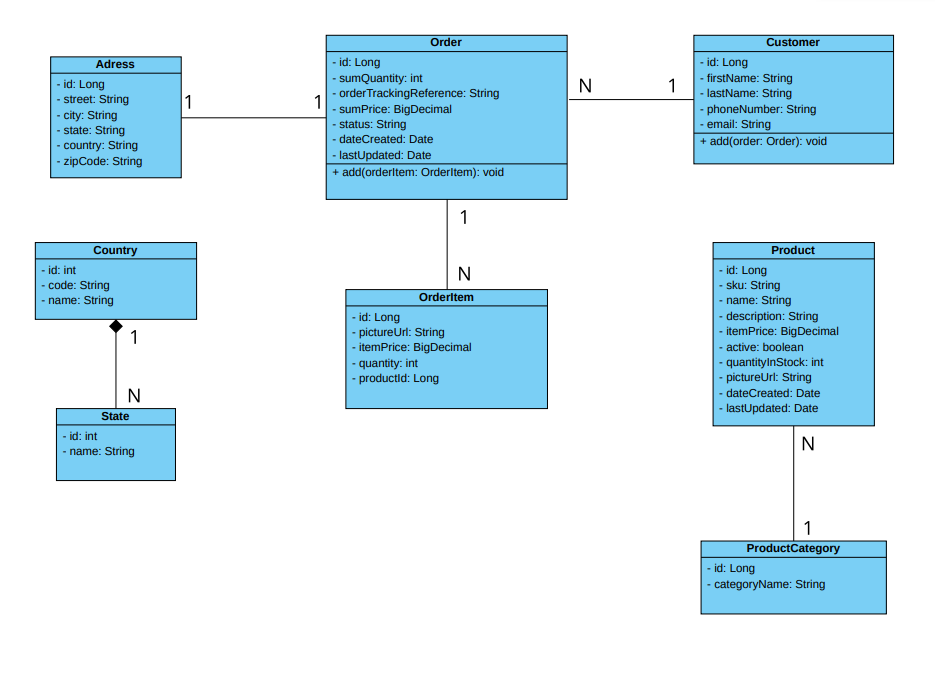
\includegraphics[width=\textwidth]{images/ClassDiagram.png}
	\caption{Klassendiagram für die Ecommerce Anwendung ShopNook}
	\label{fig:class_diagram}
\end{figure}

\subsection{Use-Case Diagramme}\index{Use-Case Diagramme}


\section{Front-End Technologien}\index{Front-End Technologien}

Dieses Kapitel befasst sich mit Front-End-Technologien wie HTML, CSS, Typescript und Angular, die für die Erstellung interaktiver, reaktionsfähiger und visuell ansprechender Benutzeroberflächen in unserer E-Commerce-Anwendung unerlässlich sind.

\subsection{HTML/CSS}\index{HTML/CSS}

HTML and CSS sind die grundlegenden Technologien zur Erstellung und Gestaltung von Webseiten. HTML liefert die Struktur und den Inhalt einer Webseite, während CSS für die visuelle Darstellung, Layout, Farben und Schriftarten, verwendet wird. Sie ermöglichen es optisch ansprechende und gut strukturierte Webseiten zu erstellen \cite{HTML/CSS:2024}.

\subsection{Typescript}\index{Typescript}

TypeScript\footnote{https://www.typescriptlang.org} ist eine stark typisierte Programmiersprache, die auf JavaScript aufbaut und statische Typdefinitionen hinzufügt. Sie soll die Entwicklung umfangreicher Anwendungen überschaubarer machen, indem sie es den Entwicklern ermöglicht, Fehler schon früh im Entwicklungsprozess zu erkennen, wodurch Fehler reduziert und die Codequalität verbessert werden. \cite{Typescript:2024}.\\
Die wichtigsten Vorteile von TypeScript sind:
\begin{itemize}
	\item \textbf{Statische Typisierung:} Die statische Typisierung  ermöglicht es Entwicklern, Variablentypen explizit zu definieren, was zu einer besseren Tooling-Unterstützung führt, z. B. bei der Code-Vervollständigung und beim Refactoring. Es hilft auch bei der Identifizierung von typbezogenen Fehlern während der Kompilierungszeit und nicht zur Laufzeit.
	\item \textbf{Wartbarkeit:} Durch die Hinzufügung von Typdefinitionen wird der Code selbstdokumentierender und leichter verständlich, was in großen Codebasen, in denen mehrere Entwickler zusammenarbeiten, entscheidend ist.
\end{itemize}
Durch die Wahl von TypeScript für das ShopNook-Projekt wurde es sichergestellt, dass das Frontend der Anwendung robust, wartbar und skalierbar ist und die hohen Anforderungen an eine professionelle E-Commerce-Plattform erfüllt.

\subsection{Angular}\index{Angular}

Angular\footnote{https://angular.io} ist ein Open-Source-Framework für Webanwendungen, das von Google entwickelt und gepflegt wird. Es wird für die Erstellung dynamischer, einseitiger Anwendungen (SPAs) mit TypeScript und HTML verwendet. Das Framework bietet eine robuste Plattform für die Entwicklung komplexer Anwendungen, indem es einen umfassenden Satz von Tools und Funktionen wie Datenbindung, Dependency Injection und eine modulare Architektur bietet \cite{Angular:2024}.\\
Eine der Hauptstärken von Angular ist seine komponentenbasierte Struktur, die es Entwicklern ermöglicht, wiederverwendbare UI-Komponenten zu erstellen, die die Wartbarkeit und Skalierbarkeit verbessern. Darüber hinaus bietet Angular leistungsstarke Funktionen wie reaktive Programmierung mit RxJS\footnote{https://rxjs.dev}, Zustandsverwaltung und ein reichhaltiges Ökosystem von Bibliotheken, was es zu einer idealen Wahl für Anwendungen auf Unternehmensebene macht.

\subsubsection{Komponentenbasierte Architektur}

Die komponentenbasierte Architektur von Angular gliedert die Anwendung in kleine, in sich geschlossene Einheiten, die als Komponenten bezeichnet werden. Jede Komponente kapselt einen bestimmten Teil der Benutzeroberfläche (UI) und die damit verbundene Logik \cite{Angular2:2024}.\\
Komponenten sind die wichtigsten Bausteine für Angular-Anwendungen. Wie es in der Abbildung \ref{a1} bezeichnet wurde besteht jede Komponente aus: 

\begin{figure} [h]
	\centering
	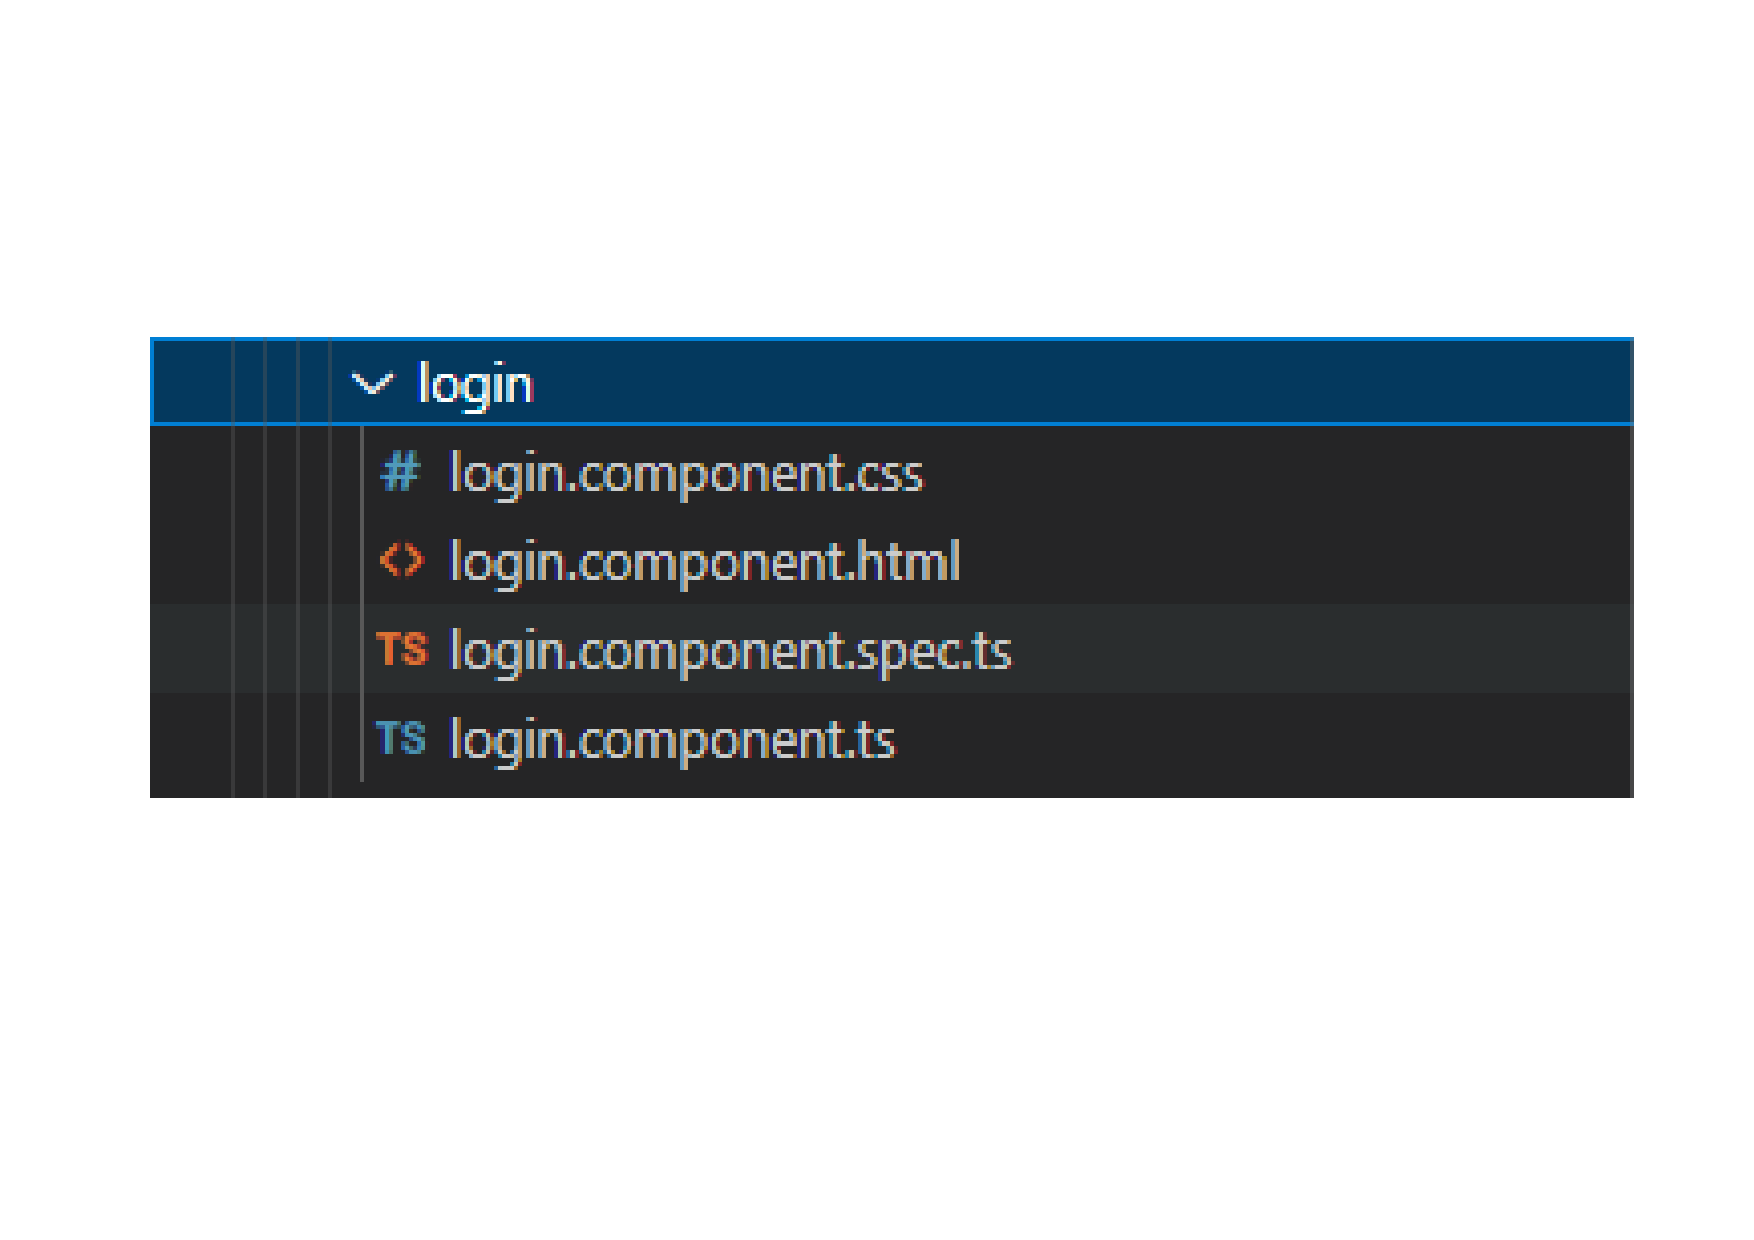
\includegraphics[scale=0.30]{images/Components.pdf}
	\caption{Beispielhafte Dateistruktur einer Angular-Anwendung mit verschiedenen Komponenten}
	\label{a1}
\end{figure}

\begin{itemize}
	\item einer Komponentendatei \texttt{<component-name>.component.ts}
	\item einer Vorlagedatei \texttt{<component-name>.component.html}
	\item einer CSS-Datei \texttt{<component-name>.component.css}
	\item Einer Datei mit Prüfvorschriften \texttt{<component-name>.component.spec.ts}
\end{itemize}


Dieser modulare Ansatz bringt mit sich mehrere Vorteile wie Wiederverwendbarkeit und Wartbarkeit.

\subsubsection{Single Page Application (SPA)}

Angular eignet sich besonders gut für die Erstellung von Single Page Applications (SPAs). In einer SPA lädt die gesamte Anwendung eine einzige HTML-Seite und aktualisiert den Inhalt dynamisch, wenn der Benutzer mit der Anwendung interagiert, ohne dass eine komplette Seite neu geladen werden muss \cite{Angular3:2024}. \\
Dieser Ansatz bietet mehrere Vorteile:
\begin{itemize}
	\item \textbf{Verbesserte Benutzerfreundlichkeit:} SPAs bieten eine reibungslosere und schnellere Benutzererfahrung, da nur die notwendigen Teile der Seite aktualisiert werden, anstatt die gesamte Seite neu zu laden.
	\item \textbf{Geringere Serverlast:} Sie entlasten den Server, da weniger Ganzseitenanfragen gestellt werden, was zu einer effizienteren Nutzung der Serverressourcen führt.
\end{itemize}

Durch die Nutzung der komponentenbasierten Architektur und der SPA-Funktionen von Angular kann die Anwendung ShopNook eine nahtlose und reaktionsschnelle Benutzererfahrung bieten, die für die Kundenbindung und -zufriedenheit entscheidend ist.


%\subsubsection{Document Object Model (DOM)}
\section{Back-End Technologien}\index{Back-End Technologien}

In diesem Kapitel werden Back-End-Technologien untersucht, wobei der Schwerpunkt auf Spring Boot liegt, um robuste, skalierbare und sichere serverseitige Logik und APIs für unsere E-Commerce-Anwendung zu erstellen.

\subsection{Java}\index{Java}

Java ist eine weit verbreitete Programmiersprache, die für ihre Plattformunabhängigkeit, Stabilität und umfassende Bibliotheken bekannt ist. Aufgrund ihrer Vielseitigkeit und Leistung wird Java häufig für die Entwicklung von Back-End-Anwendungen verwendet \cite{Java:2024}. In der E-Commerce-Anwendung (ShopNook) wird Java genutzt, um eine robuste und skalierbare serverseitige Logik zu gewährleisten.

\subsection{REST-API}\index{REST-API}

REST ist ein Architekturstil für die Entwicklung vernetzter Anwendungen. Er basiert auf einem zustandslosen, Client-Server- und cachefähigen Kommunikationsprotokoll, und in fast allen Fällen wird das HTTP-Protokoll verwendet. REST-APIs sind so konzipiert, dass sie einfach, leichtgewichtig und skalierbar sind, was sie zu einer beliebten Wahl für Webdienste macht \cite{REST:2024}.

\subsubsection{Einführung in REST}
Angelehnt an \cite{REST:2024} bieten REST-APIs eine Möglichkeit, über HTTP auf die Funktionalität und Daten einer Anwendung zuzugreifen. Sie folgen den Prinzipien von REST, die auf Ressourcen und deren Repräsentationen basieren. Jede Ressource wird durch eine eindeutige URI identifiziert und kann durch standardisierte HTTP-Methoden manipuliert werden:
\begin{itemize}
	\item GET: Abrufen von Ressourcen
	\item POST: Erstellen neuer Ressourcen
	\item PUT: Aktualisieren bestehender Ressourcen
	\item DELETE: Löschen von Ressourcen
\end{itemize}

REST-APIs sind also aufgrund ihrer Architektur und Funktionsweise weit verbreitet und bieten eine Reihe von Vorteilen:

\begin{itemize}
	\item \textbf{Skalierbarkeit:} Durch das stateless Design können REST-APIs leicht skaliert werden. Jeder HTTP-Request enthält alle notwendigen Informationen, um ihn zu verarbeiten, ohne dass der Server den vorherigen Zustand kennen muss.
	\item \textbf{Flexibilität:} REST-APIs sind flexibel und können mit verschiedenen Datenformaten arbeiten. JSON ist das gebräuchlichste Format, da es leichtgewichtig und gut lesbar ist.
	\item \textbf{Interoperabilität:\footnote{Interoperabilität ist die Fähigkeit verschiedener Systeme oder Software, zusammenzuarbeiten und Informationen nahtlos auszutauschen\cite{wiki:listing}.}} REST-APIs nutzen standardisierte HTTP-Methoden, was ihre Interoperabilität mit verschiedenen Clients und Plattformen gewährleistet.
	\item \textbf{Leichte Integration:} REST-APIs lassen sich leicht in bestehende Systeme integrieren, da sie auf bekannten Webstandards basieren.
\end{itemize}

Um die Sicherheit von REST-APIs in der ShopNook-Plattform weiter zu gewährleisten, spielt die Implementierung von HTTPS in Kombination mit SSL/TLS eine entscheidende Rolle, da diese Technologien eine sichere und verschlüsselte Kommunikation zwischen dem Client und dem Server ermöglichen.

\subsection{HTTPS und SSL/TLS}

HTTPS ist die sichere Version von HTTP, dem Protokoll, über das die Daten zwischen dem Browser des Kunden und der Website, mit der er verbunden ist, gesendet werden. Das „S“ am Ende von HTTPS steht für „Secure“, was bedeutet, dass die gesamte Kommunikation zwischen dem Kunden und dem Server verschlüsselt ist \cite{HTTPS:2024}.\\
SSL/TLS sind allerdings Verschlüsselungsprotokolle, die eine sichere Kommunikation über ein Computernetz ermöglichen. SSL war das ursprüngliche Protokoll, aber es wurde zugunsten von TLS, das sicherer und effizienter ist, veraltet \cite{SSL/TLS:2023}. Diese Protokolle bieten mehrere wichtige Sicherheitsfunktionen, die im Folgenden näher erläutert werden:

\begin{itemize}
	\item \textbf{Verschlüsselung der Daten:} SSL und TLS verschlüsseln die zwischen dem Client und dem Server übertragenen Daten und stellt sicher, dass die Daten, selbst wenn sie abgefangen werden, nicht von Unbefugten gelesen werden können.
	\item \textbf{Server-Authentifizierung:} Diese Protokolle überprüfen auch die Identität des Servers und stellen sicher, dass die Clients mit einem legitimen Server und nicht mit einem Betrüger kommunizieren.
	\item \textbf{Datenintegrität:} Sie bieten auch Datenintegrität, indem es sicherstellt, dass die Daten während der Übertragung nicht manipuliert wurden.
\end{itemize}
In der Anwendung wurde eine HTTPS Konfiguration (siehe \ref{HTTPS-Config}) erstellt, um eine sichere Kommunikation zwischen Clients und dem Server zu gewährleisten. Dazu wurde der Server so eingestellt, dass er auf Port 8443 auf HTTPS-Datenverkehr wartet.\\
Der Konfigurationsprozess beinhaltete die Aktivierung der SSL-Unterstützung, die für die Verschlüsselung der über das Netzwerk ausgetauschten Daten unerlässlich ist.\\
Eine Keystore-Datei im PKCS12-Format \verb*|shopnook-keystore.p12| wurde verwendet, in der die für die Verschlüsselung erforderlichen SSL/TLS-Zertifikate sicher gespeichert sind. Der Keystore ist durch ein Passwort geschützt \textbf{(server.ssl.key-store-password=secret)}, so dass der Zugriff auf die kryptografischen Schlüssel nur autorisierten Prozessen vorbehalten ist. \\ 
Innerhalb des Schlüsselspeichers wird das Zertifikat durch den Alias \textbf{shopnook} identifiziert, auf den in der Konfiguration verwiesen wird, um die SSL-Vorgänge des Servers mit dem richtigen Zertifikat zu verknüpfen. Diese Einrichtung stellt sicher, dass alle zwischen dem Client und dem Server übertragenen Daten verschlüsselt werden, was einen robusten Schutz gegen Abhör- und Man-in-the-Middle-Angriffe bietet.\\
Darüber hinaus ermöglicht die Konfiguration eine einfache Anpassung an unterschiedliche Umgebungen. So kann beispielsweise der Port der Anwendung je nach Einsatzumgebung geändert werden, indem die Eigenschaft \textbf{server.port} angepasst wird. Für die QA-Demo-Umgebung ist der Port auf \textbf{9898} eingestellt, der durch Umschalten der Kommentarzeilen aktiviert werden kann.\\
Durch die sorgfältige Konfiguration dieser SSL-Einstellungen stellen wir sicher, dass ShopNook den Industriestandards für Sicherheit entspricht.\newpage

\begin{lstlisting}[language=, label=HTTPS-Config, caption={Implementierung von HTTPS und SSL Konfiguration}, ]
	#####
	#
	# HTTPS configuration
	#
	#####
	#Define the web server's listening port for HTTPS traffic
	server.port=8443 
	
	#QA Demo Port
	#server.port=9898
	
	#Activate SSL support to secure the application with HTTPS
	server.ssl.enabled=true
	
	#Specify the key alias used within the keystore for SSL
	server.ssl.key-alias=shopnook
	
	#Keystore path
	server.ssl.key-store=classpath:shopnook-keystore.p12
	
	#Password to unlock the keystore and access the SSL keys
	server.ssl.key-store-password=secret
	
	#format of the keystore file
	server.ssl.key-store-type=PKCS12
\end{lstlisting}



Durch die Implementierung von HTTPS mit SSL/TLS hält sich ShopNook an die Industriestandards für Datensicherheit, um seine Nutzer zu schützen und das Vertrauen zu erhalten. Dies ist ein entscheidender Aspekt des Backends der Anwendung, insbesondere für die Wahrung der Vertraulichkeit und Integrität sensibler Daten bei Transaktionen.

\subsection{Spring Boot}\index{Spring Boot}

Spring Boot ist ein Framework, das auf dem Spring Framework aufbaut und speziell entwickelt wurde, um schnelle, effiziente und skalierbare Anwendungen zu erstellen. Es bietet eine Vielzahl von Features, die den Entwicklungsprozess beschleunigen und vereinfachen, insbesondere für Java-basierte Webanwendungen und Microservices \cite{Spring-Framework:o.J}.

\subsubsection{Warum wurde Spring Boot ausgewählt ?}
Spring Boot wurde im Rahmen dieses Projekts aufgrund der breiten Unterstützung in der Entwicklergemeinde ausgewählt. Hier sind einige der Hauptgründe:
\begin{itemize}
	\item \textbf{Produktivität:} Das Framework ermöglicht es auf das Schreiben von Geschäftslogik zu konzentrieren, anstatt sich um die Konfiguration von Technologien zu kümmern.
	\item \textbf{Microservices:} Es eignet sich hervorragend für die Entwicklung von Microservices-Architekturen, indem es Server wie Tomcat bietet, sodass die Anwendungen ohne externen Server laufen können.
	\item \textbf{Integration:} Es lässt sich nahtlos in andere Spring-Projekte und eine Vielzahl von Datenbanken integrieren.
\end{itemize}
Das Framework bietet auch viele Funktionalitäten, die es von anderen abheben. Es hat viele weitere Vorteile, die hier genannt werden:

\begin{itemize}
	\item \textbf{Auto-Konfiguration:} Die Autokonfigurationsfunktion von Spring Boot konfiguriert Ihre Anwendung automatisch anhand der Abhängigkeiten, die Sie dem Projekt hinzugefügt haben. Dadurch wird die Notwendigkeit einer manuellen Konfiguration minimiert und die Entwicklung beschleunigt.
	\item \textbf{Eigenständige Anwendungen:} Spring Boot-Anwendungen können als eigenständige Java-Anwendungen verpackt werden, was die Bereitstellung einfacher und konsistenter macht.
	\item \textbf{Produktionstaugliche Funktionen:} Das Framework umfasst zahlreiche produktionsreife Funktionen wie Zustandsprüfungen, Metriken und externalisierte Konfiguration.	
\end{itemize}

\subsubsection{Wie funktionniert Spring Boot ?}

\begin{enumerate}
	\item \textbf{Initial Setup:} Mit Spring Initializr kann man schnell ein neues Spring Boot-Projekt mit allen erforderlichen Abhängigkeiten und Konfigurationen initialisieren.
	\item \textbf{Main Application Class:} Jede Spring Boot-Anwendung hat eine Hauptklasse, die mit @SpringBootApplication annotiert ist. Diese Annotation ist eine Kombination aus @Configuration, @EnableAutoConfiguration und @ComponentScan.
	\begin{lstlisting}[language=Java, caption={Main-Application-Class-Implementierung in Java}\label{mainClass.java}]
@SpringBootApplication
public class SpringBootEcommerceApplication {	
	public static void main(String[] args) {
		SpringApplication.run(SpringBootEcommerceApplication.class, args);
	}
}		
	\end{lstlisting}
	\item \textbf{Application Properties:} Spring Boot ermöglicht eine einfache Konfiguration durch application.properties-Datei. Dadurch wird die Konfiguration externalisiert, was die Verwaltung verschiedener Umgebungen erleichtert.
	\begin{lstlisting}[language=Java, caption={Implementierung von Application.properties Datei}\label{Application.properties}]
spring.datasource.driver-class-name=com.mysql.cj.jdbc.Driver
spring.datasource.url=jdbc:mysql://localhost:3306/full-stack-ecommerce?
useSSL=false&useUnicode=yes&characterEncoding=UTF-8&allowPublicKeyRetrieval=
true&serverTimezone=UTC
spring.datasource.username=username
spring.datasource.password=password
spring.jpa.properties.hibernate.dialect=org.hibernate.dialect.MySQL8Dialect
spring.data.rest.base-path=/api
	\end{lstlisting}
\end{enumerate}

\subsubsection{Spring Security}

Spring Security ist ein robustes und anpassungsfähiges Framework, das für die Authentifizierung und Zugriffskontrolle entwickelt wurde und sich zum Standard für die Absicherung von mit Spring erstellten Anwendungen entwickelt hat.

Spring Security ist ein Framework, das sowohl die Authentifizierung als auch die Autorisierung von Java-Anwendungen übernimmt. Seine Stärke liegt in der Flexibilität, die es erlaubt, es leicht zu erweitern, um spezifische Anforderungen zu erfüllen.

Das Framework bietet eine Reihe von Funktionen, darunter umfassende Unterstützung für Authentifizierung und Autorisierung, Schutz vor verschiedenen Angriffen wie Session Fixation, Clickjacking und Cross-Site Request Forgery, Integration mit der Servlet API und optionale Kompatibilität mit Spring Web MVC \cite{Spring-Security:o.J}.

Zum Schutz der Endpunkte für Kundenbestellungen wurde Spring Security mit OAuth2-Authentifizierung implementiert, wobei JWT zur Gewährleistung eines sicheren Zugriffs verwendet wird. Die Einrichtung umfasste die Konfiguration von CORS zur Verwaltung von Herkunftsübergreifenden Anfragen und die Anpassung von Sicherheitseinstellungen wie die Deaktivierung des CSRF-Schutzes und die Handhabung der Inhaltsaushandlung. Dieser Ansatz gewährleistet robuste Sicherheit, während er verschiedene Inhaltstypen unterstützt und die gemeinsame Nutzung von Ressourcen über verschiedene Ursprünge hinweg effektiv handhabt.

\subsection{Stripe API}
In diesem Teil wird die Stripe-API näher beleuchtet, beginnend mit einem Überblick über ihre grundlegenden Funktionen und Hauptmerkmale. Anschließend wird die Integration der API in unsere Anwendung beschrieben, gefolgt von spezifischen Anwendungsfällen, die die Vielseitigkeit von Stripe in unserem Projekt veranschaulichen. Diese Analyse zeigt, wie Stripe eine nahtlose und sichere Zahlungsabwicklung ermöglicht.
\subsubsection{Überblick}

Die Stripe-API bietet ein umfassendes Paket von Tools für Entwickler zur Integration und Interaktion mit den Diensten von Stripe. Sie wurde nach REST-Prinzipien mit vorhersehbaren, ressourcenorientierten URLs entwickelt. Anfragen werden mit verschlüsseltem Form Körpern gesendet, und Antworten werden im JSON-Format zurückgegeben. Je nach verwendetem API-Schlüssel kann die Stripe-API entweder im Testmodus oder im Live-Modus betrieben werden. Verschiedene Stripe-Konten können je nach Version und benutzerdefinierten Funktionen unterschiedliche API-Funktionen aufweisen. Die API-Referenz enthält Codebeispiele für die Integration in verschiedenen Programmiersprachen\cite{Stripe-API:o.J}.

\subsubsection{Hauptmerkmale der Stripe API}
Zu den wichtigsten Funktionen der Stripe-API gehören:

\begin{itemize}
	\item Die API bearbeitet Anfragen einzeln, ohne Unterstützung für Massenaktualisierungen, pro Anfrage kann nur ein Objekt aktualisiert werden.
	\item Die Funktionalität kann sich mit jeder neuen Version der API ändern, wenn Updates veröffentlicht werden.
	\item Die Stripe-API unterstützt eine breite Palette von Zahlungsmethoden, darunter Karten, digitale Geldbörsen, Bankabbuchungen und -überweisungen sowie Bankumleitungen, zusammen mit Optionen wie „Sofort kaufen, später bezahlen“ und bargeldbasierten Gutscheinen.
	\item Sie bietet Funktionen zur Umsatzoptimierung, einschließlich Tools für Authentifizierung, Autorisierung, Betrugsprävention, Streitfallmanagement und Abgleich.
	\item Stripe bietet auch Berichts- und Analysetools wie Stripe Sigma für detaillierte Einblicke und das Stripe Dashboard für das Zahlungsmanagement\cite{Stripe-API:o.J}.
\end{itemize}

\subsubsection{Stripe API Integration für nahtlose Zahlungsabwicklung}

\textbf{Integration:} \\


In der Anwendung wurde die Stripe-API sowohl in das Frontend als auch in das Backend integriert, um eine sichere und effiziente Zahlungsabwicklung zu ermöglichen. Auf dem Frontend wurde die Stripe API Version „8.179“ in der Visual Studio Code Umgebung installiert. Der \texttt{stripePublishableKey} wurde eingebunden, um die Funktionalität von Stripe im Frontend zu aktivieren. Außerdem wurde die Stripe.js-Bibliothek durch Hinzufügen des folgenden Skripts eingebunden:

\begin{lstlisting}[language=HTML, basicstyle=\ttfamily\small, frame=single, backgroundcolor=\color{lightgray}]
	<script src="https://js.stripe.com/v3" async></script>
\end{lstlisting}

sodass die Anwendung direkt über den Browser mit der API von Stripe interagieren kann.

Am Backend wurde der geheime Schlüssel von Stripe(stripe.key.secret) sicher in der Datei application.properties der Spring Boot-Anwendung gespeichert. Dieser Schlüssel ist für die sichere Handhabung sensibler Vorgänge wie die Erstellung von Zahlungsintentionen und die Verwaltung von Transaktionen unerlässlich. Die Payment Intent API wurde im Backend zur Abwicklung des Zahlungsprozesses verwendet, um sicherzustellen, dass die Transaktionen authentifiziert, autorisiert und effizient verarbeitet werden\cite{Stripe-Intents:o.J}. \\


\noindent\textbf{Anwendungsfälle:} \\


Die Stripe API spielt eine entscheidende Rolle in verschiedenen zahlungsbezogenen Szenarien innerhalb der Anwendung. Sie wird hauptsächlich verwendet für:
\begin{itemize}
	\item \textbf{Zahlungsabwicklung:} Die Stripe-API wird verwendet, um Zahlungen sicher zu verarbeiten. Dazu gehört das Erstellen von Zahlungsabsichten im Backend mit Java in Spring Boot, das den gesamten Zahlungslebenszyklus verwaltet, von der Zahlungsauslösung bis zur Bestätigung.
	
	\item \textbf{E-Mail-Bestätigung:} Nach einem erfolgreichen Kauf wird die Stripe-API so konfiguriert, dass sie Bestätigungs-E-Mails an die Benutzer sendet, um ihnen eine Aufzeichnung ihrer Transaktion zu liefern.
	
	\item \textbf{Frontend-Zahlungsabwicklung:} Das Frontend interagiert für die Zahlungsabwicklung mit Stripe und nutzt die Stripe.js-Bibliothek, um die Zahlungsinformationen sicher zu sammeln und mit Token zu versehen, bevor sie zur weiteren Verarbeitung an das Backend gesendet werden.
\end{itemize}

Diese umfassende Integration der Stripe-API sowohl in das Frontend als auch in das Backend stellt sicher, dass alle zahlungsrelevanten Vorgänge sicher, effizient und mit einer nahtlosen Benutzererfahrung abgewickelt werden. 

\section{Datenbankstruktur}\index{Datenbankstruktur}
In diesem Abschnitt wird die Datenbankstruktur der Webanwendung untersucht, um ein umfassendes Verständnis für die Organisation, den Zugriff und die Verwaltung der Daten zu vermitteln. Der Schwerpunkt liegt auf dem relationalen Datenbankmodell und den spezifischen Technologien und Frameworks, die zur Handhabung der Datenpersistenz und der Transaktionen verwendet werden. Dabei wird MySQL als das gewählte Datenbanksystem zusammen mit Spring Data JPA für eine nahtlose Dateninteraktion untersucht. In den folgenden Unterabschnitten werden diese Aspekte im Detail behandelt, wobei relationale Datenbanken, die Auswahl von MySQL, Datenpersistenz und Transaktionsmanagement sowie die Integration von MySQL mit Spring Boot behandelt werden.
\subsection{Übersicht über relationale Datenbanken und Auswahl von MySQL}
Die Daten in einer relationalen Datenbank sind in Tabellen mit Spalten und Zeilen organisiert, und auch die Primär- und Fremdschlüssel werden verwendet, um die Beziehungen zwischen den Tabellen herzustellen. Dieser Ansatz ist ideal für E-Commerce-Anwendungen, da er komplexe Abfragen und aussagekräftige Daten verarbeiten kann. Produktlieferungen, Auftragstransaktionen und Kundendaten werden alle ordnungsgemäß verwaltet. Die Möglichkeit, Tabellen zu verknüpfen, erleichtert umfassende Analysen, einschließlich der Nachverfolgung von Kaufdatensätzen und der Bestandskontrolle, während die Einhaltung von ACID-Eigenschaften eine zuverlässige Transaktionsverarbeitung gewährleistet, die für die Auftragsabwicklung und das Zahlungsmanagement entscheidend ist. Relationale Datenbanken wie MySQL bieten die Robustheit und Konsistenz, die für einen sicheren und produktiven Online-Shopping-Betrieb erforderlich sind \cite{IBM:o.J}.

\subsection{Datenbankschemaentwurf mit Spring Data JPA}
Ziel dieses Abschnitts ist es, zu erörtern, wie Spring Data JPA den Entwurf und die Verwaltung von Datenbankschemata vereinfacht. Es wird gezeigt, wie Spring Data JPA es Entwicklern ermöglicht, Entitäten und Beziehungen innerhalb eines Datenbankschemas abzubilden und zu verwalten, und wie es die Komplexität des Datenzugriffs durch seine Repository-Schicht abstrahiert.

Spring Data JPA vereinfacht den Entwurf von Datenbankschemata, indem es Entwicklern ermöglicht, Java-Klassen mithilfe von Annotationen wie @Entity, @Id und @OneToMany auf Datenbanktabellen abzubilden. Diese Annotationen übernehmen automatisch die Schemaerstellung und -verwaltung und stellen sicher, dass die Datenbankstruktur mit dem Domänenmodell der Anwendung übereinstimmt \cite{Docs-Spring:o.J, Baeldung:o.J}.

Die Repository-Schicht in Spring Data JPA abstrahiert die Komplexität des Datenzugriffs und bietet integrierte CRUD-Operationen über Schnittstellen wie JpaRepository. Dies macht manuelle SQL-Abfragen überflüssig und rationalisiert die Datenbankinteraktionen, so dass sich die Entwickler auf die Geschäftslogik konzentrieren können \cite{Docs-Spring-JPA-Repo:o.J, Docs-Spring-JPA-QueryMethods:o.J}.

\subsection{Datenpersistenz und Transaktionen}
In diesem Abschnitt wird erläutert, wie Spring Boot und Hibernate die Datenpersistenz handhaben. Der Schwerpunkt liegt dabei auf CRUD-Operationen, der Rolle des EntityManagers und der Interaktion des Hibernate ORM mit MySQL.

CRUD-Operationen werden mit Spring Boot und Hibernate verwaltet. Der EntityManager ist in diesem Prozess von zentraler Bedeutung und ermöglicht das Erstellen, Abrufen, Aktualisieren und Löschen von Entitäten. Er verwaltet auch den Lebenszyklus von Entitäten innerhalb von Transaktionen und stellt sicher, dass Änderungen bei Bedarf ordnungsgemäß übertragen oder zurückgenommen werden  \cite{Baeldung-EntityManager:2024}.


Hibernate ORM wird verwendet, um Java-Objekte auf Datenbanktabellen abzubilden, was die Interaktion mit der MySQL-Datenbank vereinfacht. Dieses ORM-Framework macht manuelles SQL überflüssig und bietet einen objektorientierten Ansatz für Datenbankoperationen \cite{Hibernate:o.J}.


\subsection{MySQL-Workbench und SQL}
In diesem Abschnitt wird die MySQL Workbench als Werkzeug für den Entwurf und die Verwaltung von Datenbanken und SQL als Sprache für die Erstellung von Abfragen und die Verwaltung der Datenbank vorgestellt.

MySQL Workbench wurde zur Visualisierung des Datenbankschemas eingesetzt und ermöglichte eine intuitive Gestaltung und Verwaltung der Datenbankstrukturen. Sie erleichterte die Erstellung und Änderung von Tabellen, Beziehungen und Indizes. Darüber hinaus wurde SQL verwendet, um Abfragen für Tests und die Datenbankverwaltung auszuführen, einschließlich Aufgaben wie Datenmanipulation und Schemaaktualisierungen \cite{mySQL:o.J}.

\subsection{Datenbankverbindung und -konfiguration in Spring Boot}
In diesem Abschnitt wird erläutert, wie die Datenbank innerhalb der Spring Boot-Anwendung verbunden und konfiguriert wird.

Die Datenbankverbindung wird in der Datei \texttt{application.properties} konfiguriert. Zu den wichtigsten Eigenschaften gehören die JDBC-URL, der Name der Treiberklasse und die Anmeldeinformationen, wie in \hyperref[Application.properties]{Listing~2.2} dargestellt.

\section{Authentifizierungs- und Autorisierungsprotokolle}\index{Authentifizierungs- und Autorisierungsprotokolle}

In der modernen digitalen Landschaft ist die Gewährleistung eines sicheren Zugriffs auf Ressourcen von entscheidender Bedeutung. In diesem Abschnitt werden die wichtigsten Protokolle und Standards zur Verwaltung der Benutzerauthentifizierung und -autorisierung untersucht, darunter JWT, OAuth2 und OpenID Connect.

\subsection{Okta}
Okta verbindet Benutzer mit jeder Anwendung über alle Geräte hinweg. Es ist ein Cloud-basierter Identitätsmanagement-Service, der mit verschiedenen lokalen Systemen kompatibel ist. Okta bietet der IT-Abteilung die Möglichkeit, den Zugriff auf Anwendungen und Geräte über eine sichere, zuverlässige und gut geprüfte Cloud-Plattform zu verwalten, mit einer tiefen Integration in lokale Systeme und Verzeichnisse.

Okta bietet Funktionen wie Provisioning, Single Sign-On (SSO), Active Directory (AD) und LDAP-Integration, zentrales Nutzer-Deprovisioning, Multi-Faktor-Authentifizierung (MFA), mobiles Identitätsmanagement und anpassbare Sicherheitsrichtlinien. Diese Funktionen werden durch das Okta Integration Network (OIN) vereinheitlicht, das umfangreiche Integrationsoptionen bietet und SSO für alle Anwendungen ermöglicht, die Ihre Benutzer benötigen\cite{Okta:o.J}.

\subsection{JWT}

JWT ist ein offener Standard (RFC 7519) für die sichere Übertragung von Informationen in Form eines JSON-Objekts. Diese Informationen sind aufgrund der digitalen Unterzeichnung überprüfbar und vertrauenswürdig. JWTs können mit einem geheimen Schlüssel mit HMAC oder mit einem öffentlichen/privaten Schlüsselpaar mit RSA oder ECDSA signiert werden. Hier sind einige Situationen, in denen JSON-Web-Token von Vorteil sind:

\begin{itemize}
	\item \textbf{Autorisierung:}  JWTs werden in der Regel zur Authentifizierung verwendet. Nach der Anmeldung enthält jede Anfrage das JWT, das den Zugriff auf autorisierte Routen, Dienste und Ressourcen ermöglicht.
	\item \textbf{Informationsaustausch:} Mit JWTs werden Informationen sicher zwischen Parteien übertragen. Signierte JWTs bestätigen die Identität des Absenders und stellen sicher, dass der Inhalt unverändert bleibt, da die Signatur sowohl aus der Kopfzeile als auch aus der Nutzlast abgeleitet wird\cite{JWT:o.J}.
\end{itemize}

\subsection{OAuth2}
OAuth 2.0, kurz für „Open Authorization“, ist ein Standard, der es einer Website oder Anwendung ermöglicht, im Namen eines Benutzers auf Ressourcen anderer Webanwendungen zuzugreifen. Er löste 2012 OAuth 1.0 ab und hat sich seitdem zum Industriestandard für die Online-Autorisierung entwickelt. OAuth 2.0 erleichtert den autorisierten Zugriff und schränkt gleichzeitig die Aktionen ein, die eine Client-Anwendung für den Benutzer auf Ressourcen durchführen kann, ohne die Anmeldedaten des Benutzers preiszugeben\cite{OAuth2:o.J}.

\subsection{OpenID Connect}
OpenID Connect ist ein Authentifizierungsprotokoll, das auf dem OAuth 2.0 Framework (IETF RFC 6749 und 6750) aufbaut. Es rationalisiert die Überprüfung der Benutzeridentität, indem es die von einem Autorisierungsserver durchgeführte Authentifizierung nutzt und Benutzerprofilinformationen in einer RESTful und interoperablen Weise bereitstellt.

OpenID Connect fördert ein Internet-Identitäts-Ökosystem durch einfache Integration, Sicherheits- und Datenschutzfunktionen, breite Client- und Gerätehilfe und die Möglichkeit für jede Einrichtung, als OpenID Provider (OP) zu agieren\cite{OpenId:o.J}.


\section{Entwicklungsumgebung und Versionskontrolle}\index{Entwicklungsumgebung und Versionskontrolle}
In diesem Abschnitt werden die integrierten Entwicklungsumgebungen (IDEs) und Versionskontrollsysteme beschrieben, die im Rahmen des Projekts eingesetzt wurden. Er bietet einen Überblick über die für die Entwicklung ausgewählten IDEs und die Versionskontrollwerkzeuge, die zur effektiven Verwaltung von Codeänderungen eingesetzt wurden.
\subsection{Entwicklungsumgebung}
Dieser Unterabschnitt beschreibt die im Projekt verwendeten Entwicklungsumgebungen, wobei der Schwerpunkt auf IntelliJ IDEA und Visual Studio Code (VS Code) liegt. Er hebt die Funktionen und Vorteile der einzelnen IDEs bei der Unterstützung des Entwicklungsprozesses und der Steigerung der Produktivität hervor.

\subsubsection{IntelliJ IDEA}

IntelliJ IDEA ist bekannt für seinen leistungsstarken Code-Editor, der sich durch eine umfassende Anfangsindizierung beim Verstehen und Verwalten von Code auszeichnet. Diese Funktion ermöglicht es ihm, Fehler in Echtzeit zu erkennen, kontextbezogene Vorschläge zur Code-Vervollständigung anzubieten und sicheres Code-Refactoring durchzuführen, neben anderen Funktionen. Es ist mit einer umfangreichen Suite integrierter Entwicklerwerkzeuge ausgestattet und bietet robuste Unterstützung für verschiedene Spring-Frameworks sowohl in Java als auch in Kotlin. Dazu gehören Spring MVC, Spring Boot, Spring Integration, Spring Security und Spring Cloud. Zu den bemerkenswerten Vorteilen gehören intelligente Codierungshilfe, sofortige Navigation innerhalb des Spring-Codes, integrierte Entwicklungswerkzeuge und erweiterte Visualisierungsfunktionen \cite{Jetbrains:o.J}.


\subsubsection{Visual Studio Code}

 Visual Studio Code ist ein vielseitiger und effizienter Quellcode-Editor, der mit Windows, macOS und Linux kompatibel ist. Er bietet native Unterstützung für JavaScript, TypeScript und Node.js und verfügt über eine breite Palette von Erweiterungen für weitere Sprachen und Plattformen \cite{visual-studio:o.J}.

Da die Front-End-Entwicklung Angular, ein auf TypeScript basierendes Framework, nutzt, wurde Visual Studio Code als Entwicklungsumgebung gewählt. Die starke native Unterstützung für TypeScript erleichtert die effiziente und optimierte Projektentwicklung und macht zusätzliche Erweiterungen überflüssig. \cite{visualstudio-angular:o.J}.

\subsection{Versionskontrolle}
In diesem Unterabschnitt werden die im Projekt eingesetzten Versionskontrollsysteme beschrieben, wobei der Schwerpunkt auf Git und GitHub liegt. Es wird erläutert, wie diese Tools die Codeverwaltung, die Zusammenarbeit und die Verfolgung von Änderungen während des gesamten Entwicklungsprozesses erleichtert haben.
\subsubsection{Git}
Git ist ein kostenloses und quelloffenes, verteiltes Versionskontrollsystem, das entwickelt wurde, um Projekte jeder Größe schnell und effizient zu verwalten. Es hat einen minimalen Platzbedarf und liefert eine außergewöhnlich schnelle Leistung. Git übertrifft herkömmliche SCM-Tools wie Subversion, CVS, Perforce und ClearCase mit Funktionen wie kostengünstiger lokaler Verzweigung, benutzerfreundlichen Staging-Bereichen und flexiblen Arbeitsabläufen.

Eines der herausragenden Merkmale von Git ist sein Verzweigungsmodell, das es von fast allen anderen SCM-Tools unterscheidet. Git ermöglicht und fördert die Erstellung mehrerer lokaler Zweige, von denen jeder unabhängig funktionieren kann. Das Erstellen, Zusammenführen und Löschen von Zweigen geht schnell, nahtlos vonstatten und dauert oft nur Sekunden  \cite{git-scmr:o.J}.

\subsubsection{GitHub}
GitHub ist eine cloudbasierte Plattform zum Speichern, Freigeben und gemeinsamen Bearbeiten von Code. Die von Git unterstützten Kollaborationsfunktionen von GitHub ermöglichen es uns:

\begin{itemize}
	\item Projekte zu präsentieren oder zu verbreiten.
	\item Verfolgen und Verwalten von Codeänderungen im Laufe der Zeit.
	\item Andere einladen, den Code zu überprüfen und Verbesserungen vorzuschlagen.
	\item Zusammenarbeit an Projekten ohne das Risiko, dass unbeabsichtigte Änderungen die Arbeit der anderen beeinträchtigen, bis die Änderungen integriert werden können.  \cite{github:o.J}.
\end{itemize} 















\chapter{Implementierung}\label{Bausteine}

In diesem Kapitel wird die Implementierung der prinzipielle Funktionsweise der Anwendung beschrieben.
Als Grundlage für alle Seiten in der Anwendung wird ein globales Layout
\verb*|/app.component.html| angelegt, welches für alle übersetzten Seiten verwendet wird. Darin wird definiert, welche Komponenten auf jeder Seite angezeigt werden sollen.


\section{Startseite}\index{Abschnitt}\label{startseite}

Für dieses Projekt sind standardmäßig für alle Seiten die Komponenten Header, Menu, Fotter und Hauptinhalt definiert. Im Header ist eine Navigation zwischen verschiedenen Seiten, das Einloggen mit Benutzerkonto und das Suchen nach bestimmten Produkten. Der Footer zeigt weiterführende Links mit Information zum About-us, Contact-us und Help. Dazu werden als Komponenten im Ordner \verb*|/components| Komponenten wie z.B \verb*|/about-us|, \verb*|/search| oder \verb*|/product-category-menu| angelegt, in dem diese Funktionalitäten eingebaut werden.

\subsection{header}

In der Datei \verb*|/app.component.html| werden drei Komponenten im Header, wie man in \ref{listing3.1} sehen kann, aufgerufen.

\begin{lstlisting}[language=HTML, label=listing3.1 , caption=Aufruf von Header-Komponenten]
<app-search></app-search>
<app-login-state></app-login-state>
<app-cart-state></app-cart-state>
\end{lstlisting}

Das Komponent \verb*|/app-search| ist dafür zuständig, den Benutzern eine Suchfunktion bereitzustellen, mit der sie schnell und einfach nach Produkten suchen können.
In \ref{listing3.2} kann man eine HTML-Struktur der Komponente \verb*|/app-search| sehen:
\newpage

\begin{lstlisting}[language=HTML, label=listing3.2, caption=HTML-Struktur der app-search-Komponente]
<div class="search-container">
<input #searchInput class="search-input"  
type="text" placeholder="Search for products ..."
(keyup.enter)="searchProducts(searchInput.value)"/>
<button (click)="searchProducts(searchInput.value)"class="au-btn-submit">
<a href="#" class="search-btn">
<i class="fas fa-search"></i>      
</a>
</button>
</div>
\end{lstlisting}

Das Eingabefeld ist mit der Angular-Komponente über die Template Referenzvariable \verb*|#searchInput| verbunden. Benutzer können hier ihre Suchanfragen eingeben.
Die Suche kann auf zwei Arten ausgelöst werden:

\begin{enumerate}
	\item Durch Drücken der Enter-Taste: Das Ereignis \verb*|keyup.enter| ist mit der Methode \verb*|searchProducts()| verbunden, sodass die Suche gestartet wird, wenn der Benutzer die Enter-Taste drückt.
	\item Durch Klicken auf die Suchschaltfläche: Die Suche kann auch durch Klicken auf die Suchschaltfläche gestartet werden, die ebenfalls an die Methode \verb*|searchProducts()| gebunden ist.
\end{enumerate}

Die \verb*|/cart-state| bietet den Benutzern Echtzeit-Updates über den Zustand ihres Einkaufswagens, einschließlich der Gesamtanzahl der Artikel und des Gesamtpreises. Diese Komponente ermöglicht es den Benutzern, problemlos auf die Warenkorbdetails zuzugreifen und zur Kasse zu gehen oder den Inhalt ihres Warenkorbs zu ändern. Die Html-Struktur dieser Komponente wird in \ref{listing3.4} hervorgehoben: 

\begin{lstlisting}[language=, label=listing3.4, caption=HTML-Struktur der cart-state-Komponente]
<div class="cart-area">
<a routerLink = "/cart-details" class="cart-link">
<div class="cart-content">
<div class="cart-icon">
<i class="fas fa-shopping-cart"></i>
<span class="cart-quantity">{{ totalQuantity }}</span>
</div>
<div class="total-price">{{ totalPrice | currency: 'EUR' }}</div>
</div>
</a>
</div>
\end{lstlisting}

Die Komponente zeigt die Gesamtanzahl der Artikel im Warenkorb (totalQuantity) und den Gesamtpreis (totalPrice) an, die dynamisch aktualisiert werden, wenn der Benutzer mit dem Warenkorb interagiert. Sie dient auch als Link zur Warenkorbdetailseite \verb*|/cart-details|, sodass Benutzer den Inhalt ihres Warenkorbs anzeigen und ändern können.


Zusätzlich zu den Komponenten \verb*|/app-search| und \verb*|/app-cart-state| ist die Komponente \verb*|/app-login-state|, wie in \ref{listing3.1} dargestellt, für die Verwaltung des Benutzerauthentifizierungsstatus zuständig. Diese Komponente ändert ihre Anzeige dynamisch, je nachdem, ob ein Benutzer angemeldet ist oder nicht.
Die Komponente \verb*|/login-state| wurde entwickelt, um eine optimierte Benutzererfahrung zu bieten, indem sie je nach Authentifizierungsstatus des Benutzers verschiedene Optionen anzeigt. Wenn ein Benutzer nicht angemeldet ist, zeigt die Komponente eine einfache Schaltfläche „Login“ an. Wenn der Benutzer auf diese Schaltfläche klickt, wird er auf die Anmeldeseite weitergeleitet.\\
Sobald sich der Benutzer jedoch erfolgreich anmeldet, verhält sich die Komponente dynamisch, um die Benutzerinteraktion zu verbessern. Die folgenden Elemente werden angezeigt:

\begin{itemize}
	\item \textbf{Willkommensnachricht} : Eine personalisierte Nachricht heißt den Benutzer willkommen und zeigt seinen vollständigen Namen an, der vom Okta-Authentifizierungsdienst abgerufen wird.
	\item \textbf{Schaltfläche „Logout“} : Es wird eine Schaltfläche „Logout“ angezeigt, mit der Benutzer ihre Sitzung beenden und sich sicher abmelden können. Diese Schaltfläche ruft die in der Komponente definierte Funktion logout() in \verb*|/login-state.component.ts| auf, die den OktaAuth-Dienst verwendet, um den Benutzer abzumelden und die vorhandenen Token zu löschen. 
	\item \textbf{Navigations-Schaltflächen} : Zwei zusätzliche Schaltflächen, „Member“ und „Orders“, werden angezeigt, sobald der Benutzer authentifiziert ist.\\ 
	„Member“ leitet den Benutzer zur \verb*|/only-members-page.component.html|, wo er auf mitgliedsspezifische Funktionen und Informationen zugreifen kann.\\
	„Orders“ führt den Nutzer zur Seite \verb*|order-log.component.html|, wo er einen Überblick über seine bisherigen Bestellungen erhält.
\end{itemize}

\subsection{Menu}

Die Komponente \verb*|app-product-category-menu| implementiert die Seitenleiste der Anwendung, die als dynamisches Navigationsmenü fungiert. Sie ermöglicht es den Benutzern, schnell auf verschiedene Produktkategorien zuzugreifen. Die Komponente ist auf der linken Seite der Seite platziert und bleibt in der Desktop-Ansicht immer sichtbar, um eine einfache Navigation zu gewährleisten. In der \ref{listing3.6} wurde die HTML-Struktur der Komponente \verb*|app-product-category-menu| dargestellt:

\begin{lstlisting}[language=, label=listing3.6, caption=HTML-Struktur der app-product-category-menu-Komponente]
<section class="app">
<aside class="sidebar">
<header>
Menu
</header>
<nav class="sidebar-nav">
<ul class="list-unstyled navbar-list">
<li *ngFor="let tempProductCategory of productCategories">
<a routerLink="/category/{{tempProductCategory.id}}" 
routerLinkActive="active-link"> {{tempProductCategory.categoryName}}
</a>
</li>
</ul>
</nav>
</aside>
</section>
\end{lstlisting}

Die Seitenleiste \verb*|sidebar| zeigt eine Liste von Produktkategorien an, die dynamisch aus dem Backend abgerufen werden. Dies wird durch die Verwendung der Angular-Direktive \verb*|*ngFor| erreicht, die über die productCategories-Liste iteriert und für jede Kategorie ein Navigationslink erstellt.\\
Jeder Link im Navigationsmenü verwendet also die Angular-Direktive \verb*|routerLink|, um die Benutzer zu einer Seite weiterzuleiten, die Produkte in der ausgewählten Kategorie anzeigt. Der routerLinkActive-Attributwert „active-link'' wird verwendet, um den aktiven Status des Links hervorzuheben, wenn die Kategorie aktiv ist.


\section{Online-Shopping}

Der Online-Shopping-Prozess in der Anwendung besteht aus mehreren Hauptfunktionen, die alle darauf abzielen, den Benutzern ein nahtloses Einkaufserlebnis zu bieten. Dieser Prozess umfasst das Durchsuchen von Produkten, das Auswählen von Produkten, das Hinzufügen von Produkten zum Warenkorb und das Verwalten des Warenkorbs.

\subsection{Darstellung von Produkten auf der Produktseite}

Durch das Aufrufen von der Datei \verb*|/product-list-grid.component.html|, wird eine Liste der verfügbaren Produkte in einer grid-basierten oder tabellenbasierten Ansicht gezeigt. Dies ermöglicht es den Benutzern, verschiedene Produkte schnell zu durchsuchen und auszuwählen. \\
Die Produktliste, die in der Komponente \verb*|/product-list| entwickelt wurde, bietet eine visuelle Darstellung der Produkte mit einem Bild, dem Produktnamen, dem Preis und einer Schaltfläche zum Hinzufügen zum Warenkorb.

\subsection{Auswahl und Hinzufügen von Produkten zum Warenkorb}

Benutzer können Produkte auswählen, indem sie auf das Produktbild oder den Namen klicken, um zur Produktdetailseite zu navigieren. Alternativ können sie direkt das Produkt durch einen Klick auf „Add to cart'' zur Einkaufsliste hinzufügen. \verb*|addItemToCart()| (siehe \ref{listing3.11}) in der Komponente \verb*|/product-list.component.ts| wird verwendet, um ein Produkt zum Warenkorb hinzuzufügen.

\begin{lstlisting}[language=, label=listing3.11, caption=Funktion zum Hinzufügen von Produkten zum Warenkorb]
addItemToCart(myProduct: Product) {
	console.log(`Adding to the shopping cart: ${myProduct.name}, 
	${myProduct.itemPrice}`);
	const cartItem = new CartBasket(myProduct);
	this.cartService.addToCart(cartItem);
}
\end{lstlisting}

Die Funktion nimmt ein Product-Objekt als Parameter, das das ausgewählte Produkt repräsentiert und erstellt ein neues CartBasket-Objekt, das die Produktdetails enthält, und ruft \verb*|addToCart()| aus der Datei \verb*|/cart.service.ts| auf, um das Produkt zum Warenkorb hinzuzufügen.

\subsection{Warenkorbverwaltung}

Nach dem Hinzufügen von Produkten zum Warenkorb können Benutzer ihren Warenkorb verwalten, indem sie Produkte entfernen, die Menge ändern oder zur Kasse gehen.

\begin{itemize}
	\item \textbf{Produkt entfernen}: Die Funktion \verb*|removeItemFromCart|, die in \ref{listing3.12} dargestellt wurde, entfernt ein bestimmtes Produkt aus dem Warenkorb.
	\item \textbf{Menge ändern}: Die Benutzeroberfläche kann auch Steuerelemente bereitstellen, um die Menge eines bestimmten Produkts zu ändern. Diese Änderungen werden ebenfalls über die Funktion \verb*|decreaseQuantity| in \verb*|/cart-service.ts| verarbeitet (siehe \ref{listing3.12}).
\end{itemize}

\begin{lstlisting}[language=, label=listing3.12, caption=Warenkorb Service Funktionen]
remove(cartItem: CartBasket) {
	const index = this.cartItems.findIndex(cartItem => 
	cartItem.id === cartItem.id);
	
	if(index > -1)
		this.cartItems.splice(index, 1)
	
		this.calculateCartTotals();
}

decreaseQuantity(cartItem: CartBasket) {
	cartItem.quantity--;
	
	if(cartItem.quantity == 0)
	{
		this.remove(cartItem);
	}
	else
	{
		this.calculateCartTotals();
	}
}
\end{lstlisting}

\subsection{Paginierung und Suchfunktionalität}

Die Produktliste unterstützt die Paginierung und eine Suchfunktionalität, um eine große Anzahl von Produkten effizient zu handhaben.

\begin{itemize}
	\item \textbf{Paginierung}: Die Paginierung ermöglicht es den Benutzern, die Produktliste seitenweise zu durchsuchen. Die Paginierungssteuerung \verb*|ngb-pagination| aktualisiert die Anzeige basierend auf der ausgewählten Seite und der Anzahl der Elemente pro Seite.
	\item \textbf{Suchfunktionalität}: wie es in \ref{startseite} erwähnt wurde, können die Benutzer die Produktsuche verwenden, um spezifische Artikel zu finden. Die Anwendung verarbeitet die Suchanfragen, ruft die entsprechenden Produkte ab und zeigt sie auf der Seite an.
\end{itemize}

\newpage
In den Folgenden wird die implementierung der Suchfunktionalität hervorgehoben: 

\begin{lstlisting}[language=, label=listing3.13, caption=Verwaltung der Produktliste und Suche]
manageSearchProducts() {
	const myKeyword: string = this.route.snapshot.paramMap.get('keyword')!;
	
	if (this.formerKeyword != myKeyword) {
		this.pageNumber = 1;
	}
	
	this.formerKeyword = myKeyword;
	
	console.log(`keyword=${myKeyword}, pageNumber=${this.pageNumber}`);

	this.productService.searchProductsPaginated(this.pageNumber - 1,
 this.pageSize, myKeyword)
	.subscribe(this.processProductData());
}


manageProductList() {
	const hasCategoryId: boolean = this.route.snapshot.paramMap.has('id');
	
	if (hasCategoryId) {
		this.currentCategoryId = +this.route.snapshot.paramMap.get('id')!;
	} else {
		this.currentCategoryId = null;
	}
	
	if (this.previousCategoryId !== this.currentCategoryId) {
		this.pageNumber = 1;
	}
	
	this.previousCategoryId = this.currentCategoryId;
	
	console.log(`currentCategoryId=${this.currentCategoryId}, 
	pageNumber=${this.pageNumber}`);
	
	if (this.currentCategoryId !== null) {
		this.productService.getProductListPaginated(this.pageNumber - 1, 
		this.pageSize, this.currentCategoryId)
		.subscribe(this.processProductData());
	} else {
		this.productService.getAllProductsPaginated(this.pageNumber - 1, 
		this.pageSize).subscribe(this.processProductData());
	}
}
\end{lstlisting}

Das Online-Shopping-Modul der Anwendung ist so konzipiert, dass es eine benutzerfreundliche Oberfläche zum Durchsuchen, Auswählen und Verwalten von Produkten bietet. \\
Durch die Verwendung von Komponenten wie \verb*|product-list-grid.component.html| und \verb*|product-list-table.component.html| wird eine dynamische und interaktive Benutzeroberfläche geschaffen, die die Benutzererfahrung verbessert und das Einkaufen erleichtert.

\section{Bezahlprozess}\index{Formel}

In diesem Abschnitt wird der Implementierungsprozess des Bezahlvorgangs (Checkout-Prozess) beschrieben. Der Prozess umfasst mehrere Schritte, um sicherzustellen, dass Benutzer ihre Einkäufe erfolgreich abschließen können. Die Implementierung nutzt eine Kombination aus Angular-Formularen, Validierung, Stripe für die Zahlungsabwicklung und verschiedene Service-Komponenten.

\subsection{Struktur des Checkout-Formulars}

\chapter{Ergebnisse und Analyse}

Dieses Kapitel bietet einen umfassenden Überblick über die Funktionalität und die Benutzerfreundlichkeit der E-Commerce-Webanwendung, die anhand einer Reihe detaillierter Screenshots und Analysen vorgestellt wird. Es werden die wichtigsten Funktionen der Anwendung untersucht, beginnend mit dem Anmeldeprozess, der einen sicheren Benutzerzugang gewährleistet, gefolgt von den Produktsuchfunktionen, die es dem Benutzer ermöglichen, Artikel nach Schlüsselwort oder Kategorie zu finden. Der Prozess des Hinzufügens von Produkten in den Einkaufswagen, das Fortschreiten zur Kasse und das Abschließen von Zahlungen wird veranschaulicht, um die nahtlose Integration dieser wesentlichen E-Commerce-Funktionen zu demonstrieren. Darüber hinaus wird in diesem Kapitel die Funktion „Bestellhistorie“ erläutert, mit der Benutzer frühere Einkäufe überprüfen können. Auch die Seiten mit eingeschränktem Zugriff, die nur angemeldeten Benutzern zur Verfügung stehen, werden besprochen, wobei die verbesserte Benutzerfreundlichkeit und die implementierten Sicherheitsmaßnahmen hervorgehoben werden. Durch diese Elemente soll das Kapitel die Effektivität und Effizienz des Designs und der Funktionalität der Anwendung aufzeigen.

\section{Startseite}\index{Startseite}
Die Homepage der E-Commerce-Anwendung zeichnet sich durch ein schlankes und benutzerfreundliches Layout aus (siehe Abbildung \ref{fig:sample-image}).

\begin{figure}[H]  
	\centering % Centers the image
	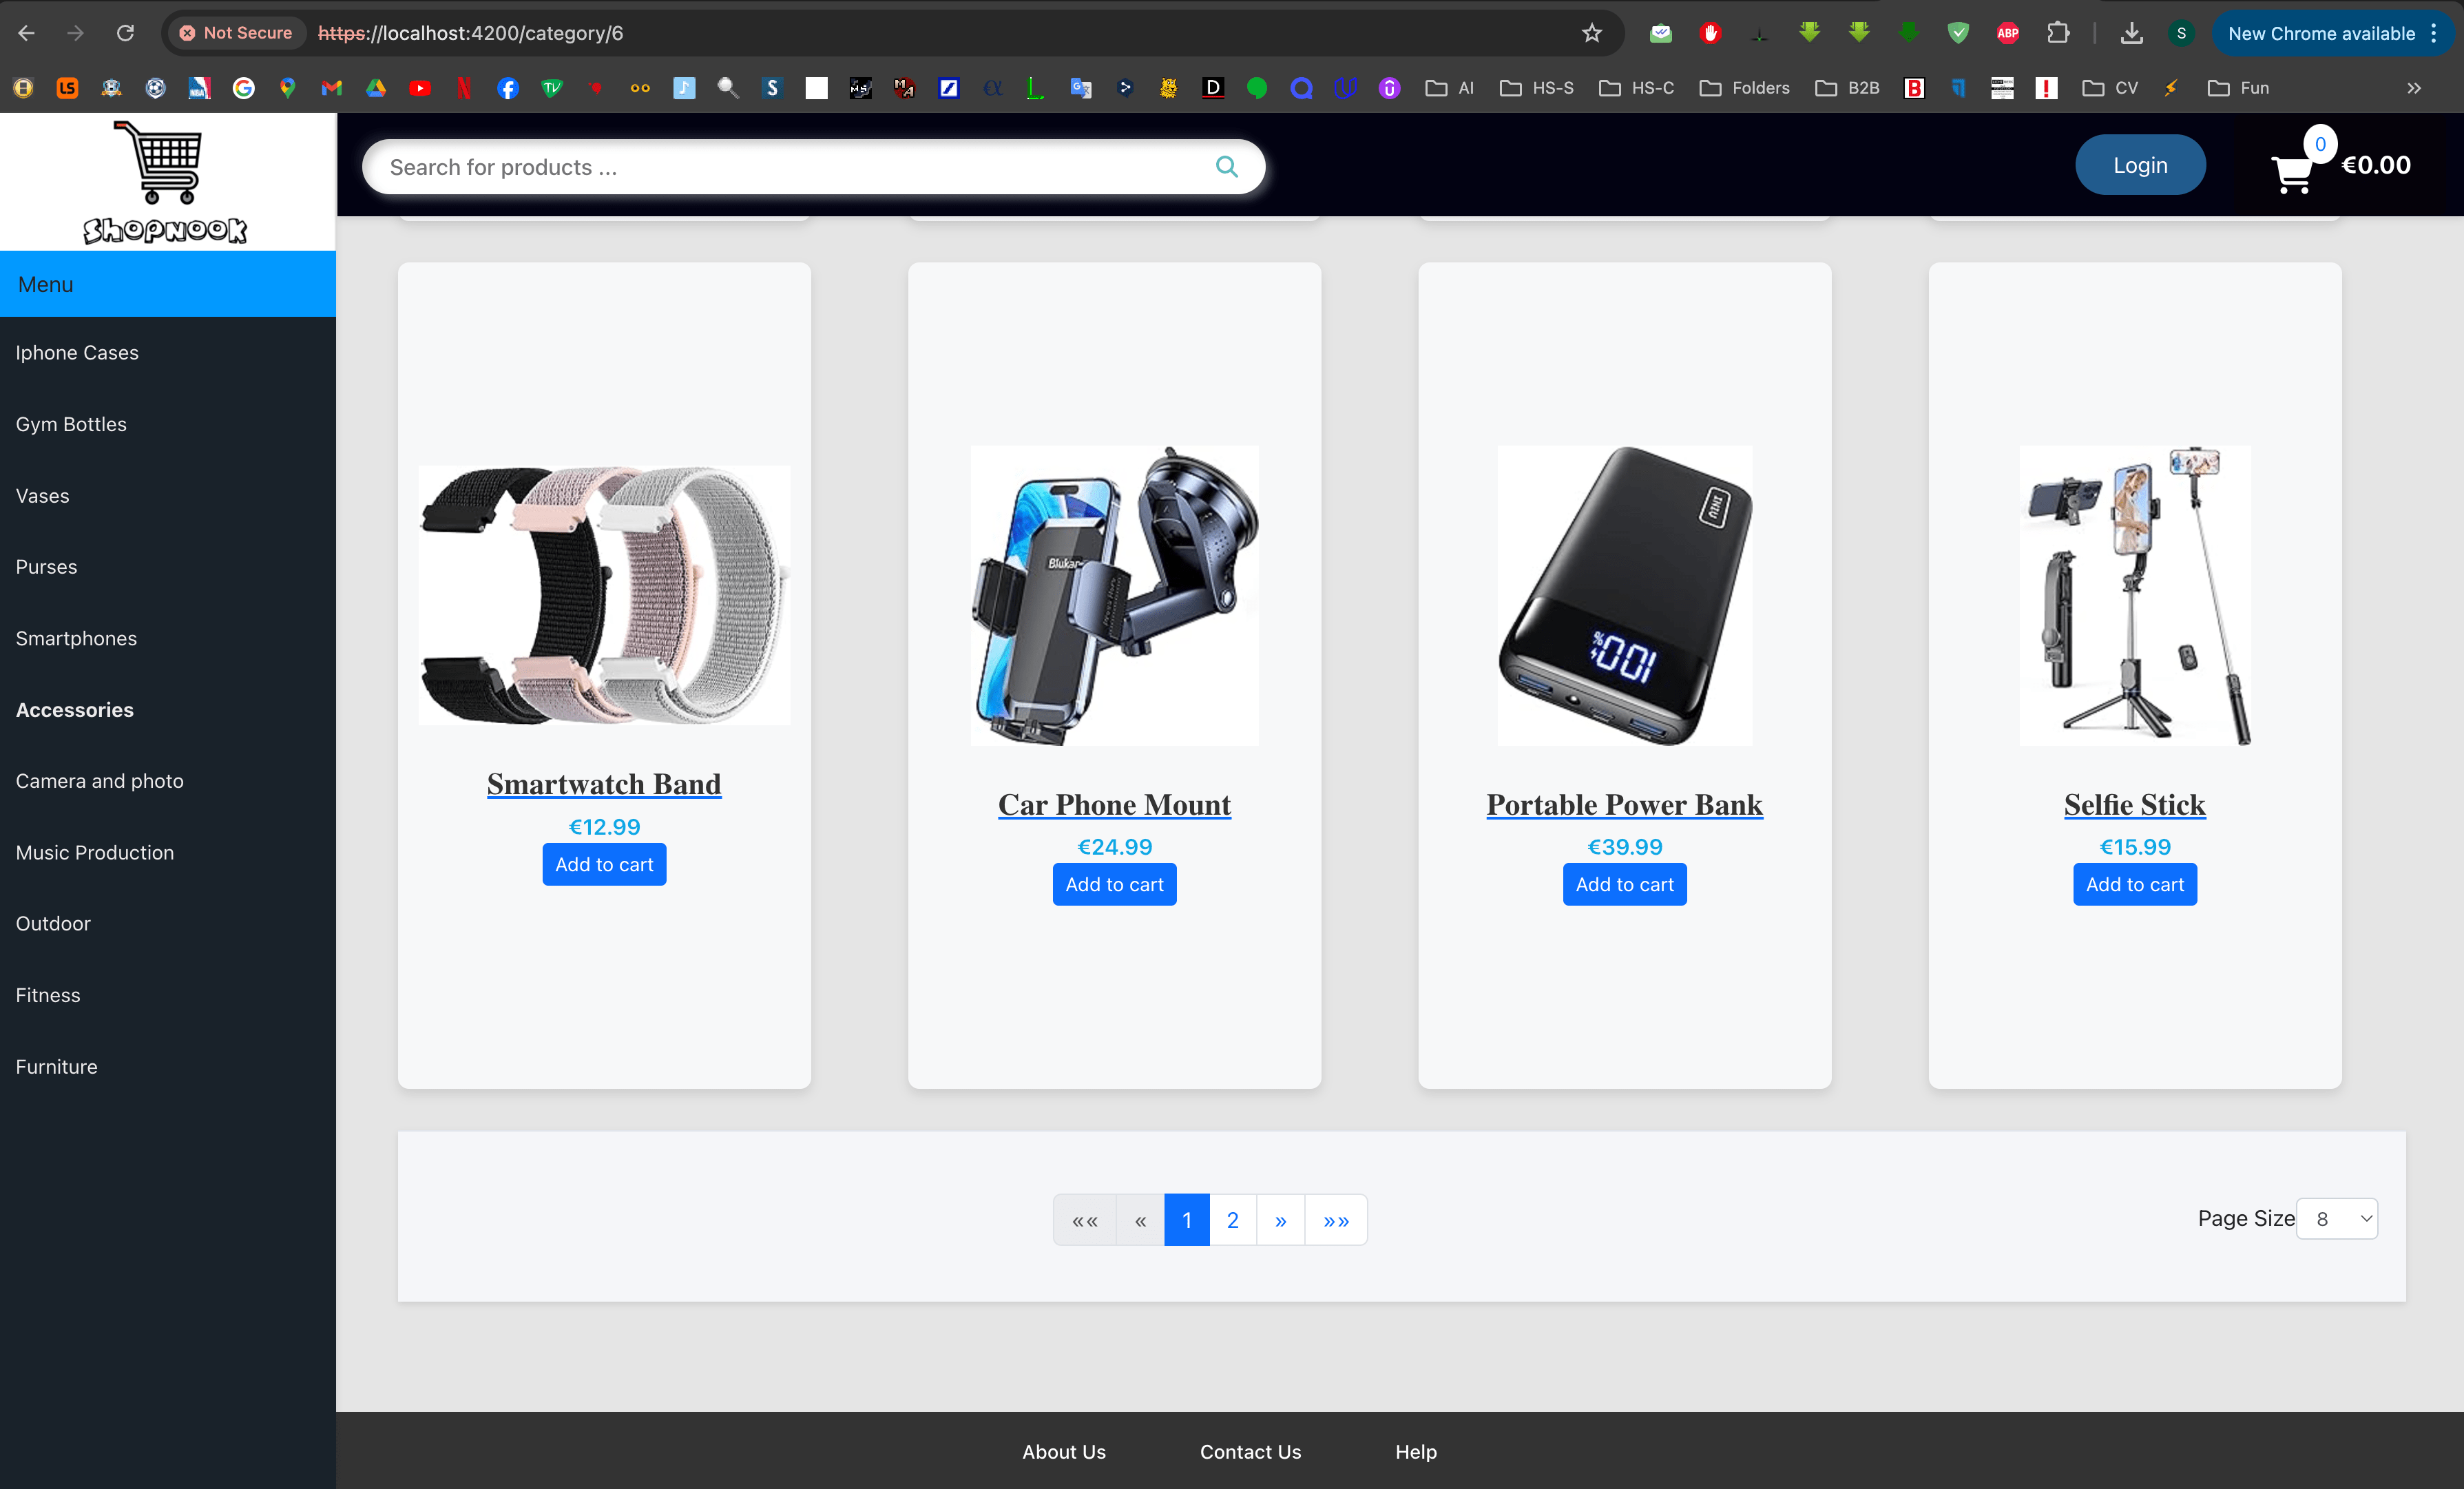
\includegraphics[width=0.9\textwidth]{Images/Home-Page.png} 
	\caption{Startseite} 
	\label{fig:sample-image} 
\end{figure}

 \subsection{Linke Seite}
 
Auf der linken Seite befindet sich:
\begin{itemize}
	\item \textbf{App-Logo:} Deutlich sichtbar auf der linken Seite, um eine gute Sichtbarkeit der Marke und eine einfache Navigation zurück zur Homepage zu gewährleisten.
	\item \textbf{Navigationsmenü:} Dieses Menü befindet sich unterhalb des Logos und bietet klare Produktkategorien, die das Surfen vereinfachen und einen schnellen Zugang zu den verschiedenen Produktbereichen ermöglichen.
\end{itemize}

 \subsection{Header}
 
In der Kopfzeile steht:
\begin{itemize}
	\item \textbf{Suchleiste:} Diese Suchleiste befindet sich am oberen Rand und ermöglicht es den Nutzern, Produkte durch die Eingabe von Schlüsselwörtern schnell zu finden, was die Effizienz der Produktsuche erhöht.
	\item \textbf{Anmeldeschaltfläche:} Diese Schaltfläche befindet sich in der Nähe der Suchleiste und bietet den Nutzern eine unkomplizierte Möglichkeit, sich in ihr Konto einzuloggen.
	\item \textbf{Warenkorb-Symbol:} Dieses Symbol befindet sich neben der Login-Schaltfläche und zeigt die Anzahl der Artikel im Warenkorb zusammen mit dem Gesamtpreis an, sodass die Nutzer einen schnellen Überblick über ihre Einkaufsaktivitäten erhalten.
\end{itemize}

 \subsection{Hauptinhalt}
Innerhalb des Hauptinhalts der Homepage gibt es:
\begin{itemize}
	\item \textbf{Produkt-Raster:} Zeigt Produkte in einem Rasterformat an, wobei jeder Eintrag gekennzeichnet ist:
	\begin{itemize}
		\item \textbf{Bild:} Bietet eine visuelle Vorschau des Produkts.
		\item \textbf{Preis:} Wird zur Transparenz deutlich angezeigt.
		\item \textbf{Titel:} Identifiziert das Produkt.
		\item \textbf{Link zu Details:} Führt den Nutzer zu einer Seite mit weiteren Informationen.
		\item \textbf{Schaltfläche „In den Warenkorb“:} Ermöglicht das schnelle Hinzufügen von Artikeln zum Einkaufswagen.
	\end{itemize}
	\item \textbf{Paginierung-Schaltflächen:} Diese Schaltflächen befinden sich am unteren Rand des Produkt-Rasters und ermöglichen es den Benutzern, durch mehrere Produktseiten zu navigieren.
\end{itemize}


 \subsection{Fußzeile}

Unten auf der Homepage gibt es Links zu
\begin{itemize}
	\item \textbf{About us:} Ein Link mit Informationen über Shopnook und sein Team.
	\item \textbf{Contact us:} Ein Link, über den Benutzer mit dem Kundendienst oder Support in Kontakt treten können.
	\item \textbf{Help:} Ein Link zu häufig gestellten Fragen oder Hilfsressourcen, die den Nutzern bei allgemeinen Fragen helfen.
\end{itemize}


\section{Warenkorb-Details}\index{Warenkorb-Details}

Die Abbildung \ref{fig:sample2-image} zeigt eine typische Schnittstelle für einen Einkaufswagen.

\begin{figure}[H]  
	\centering % Centers the image
	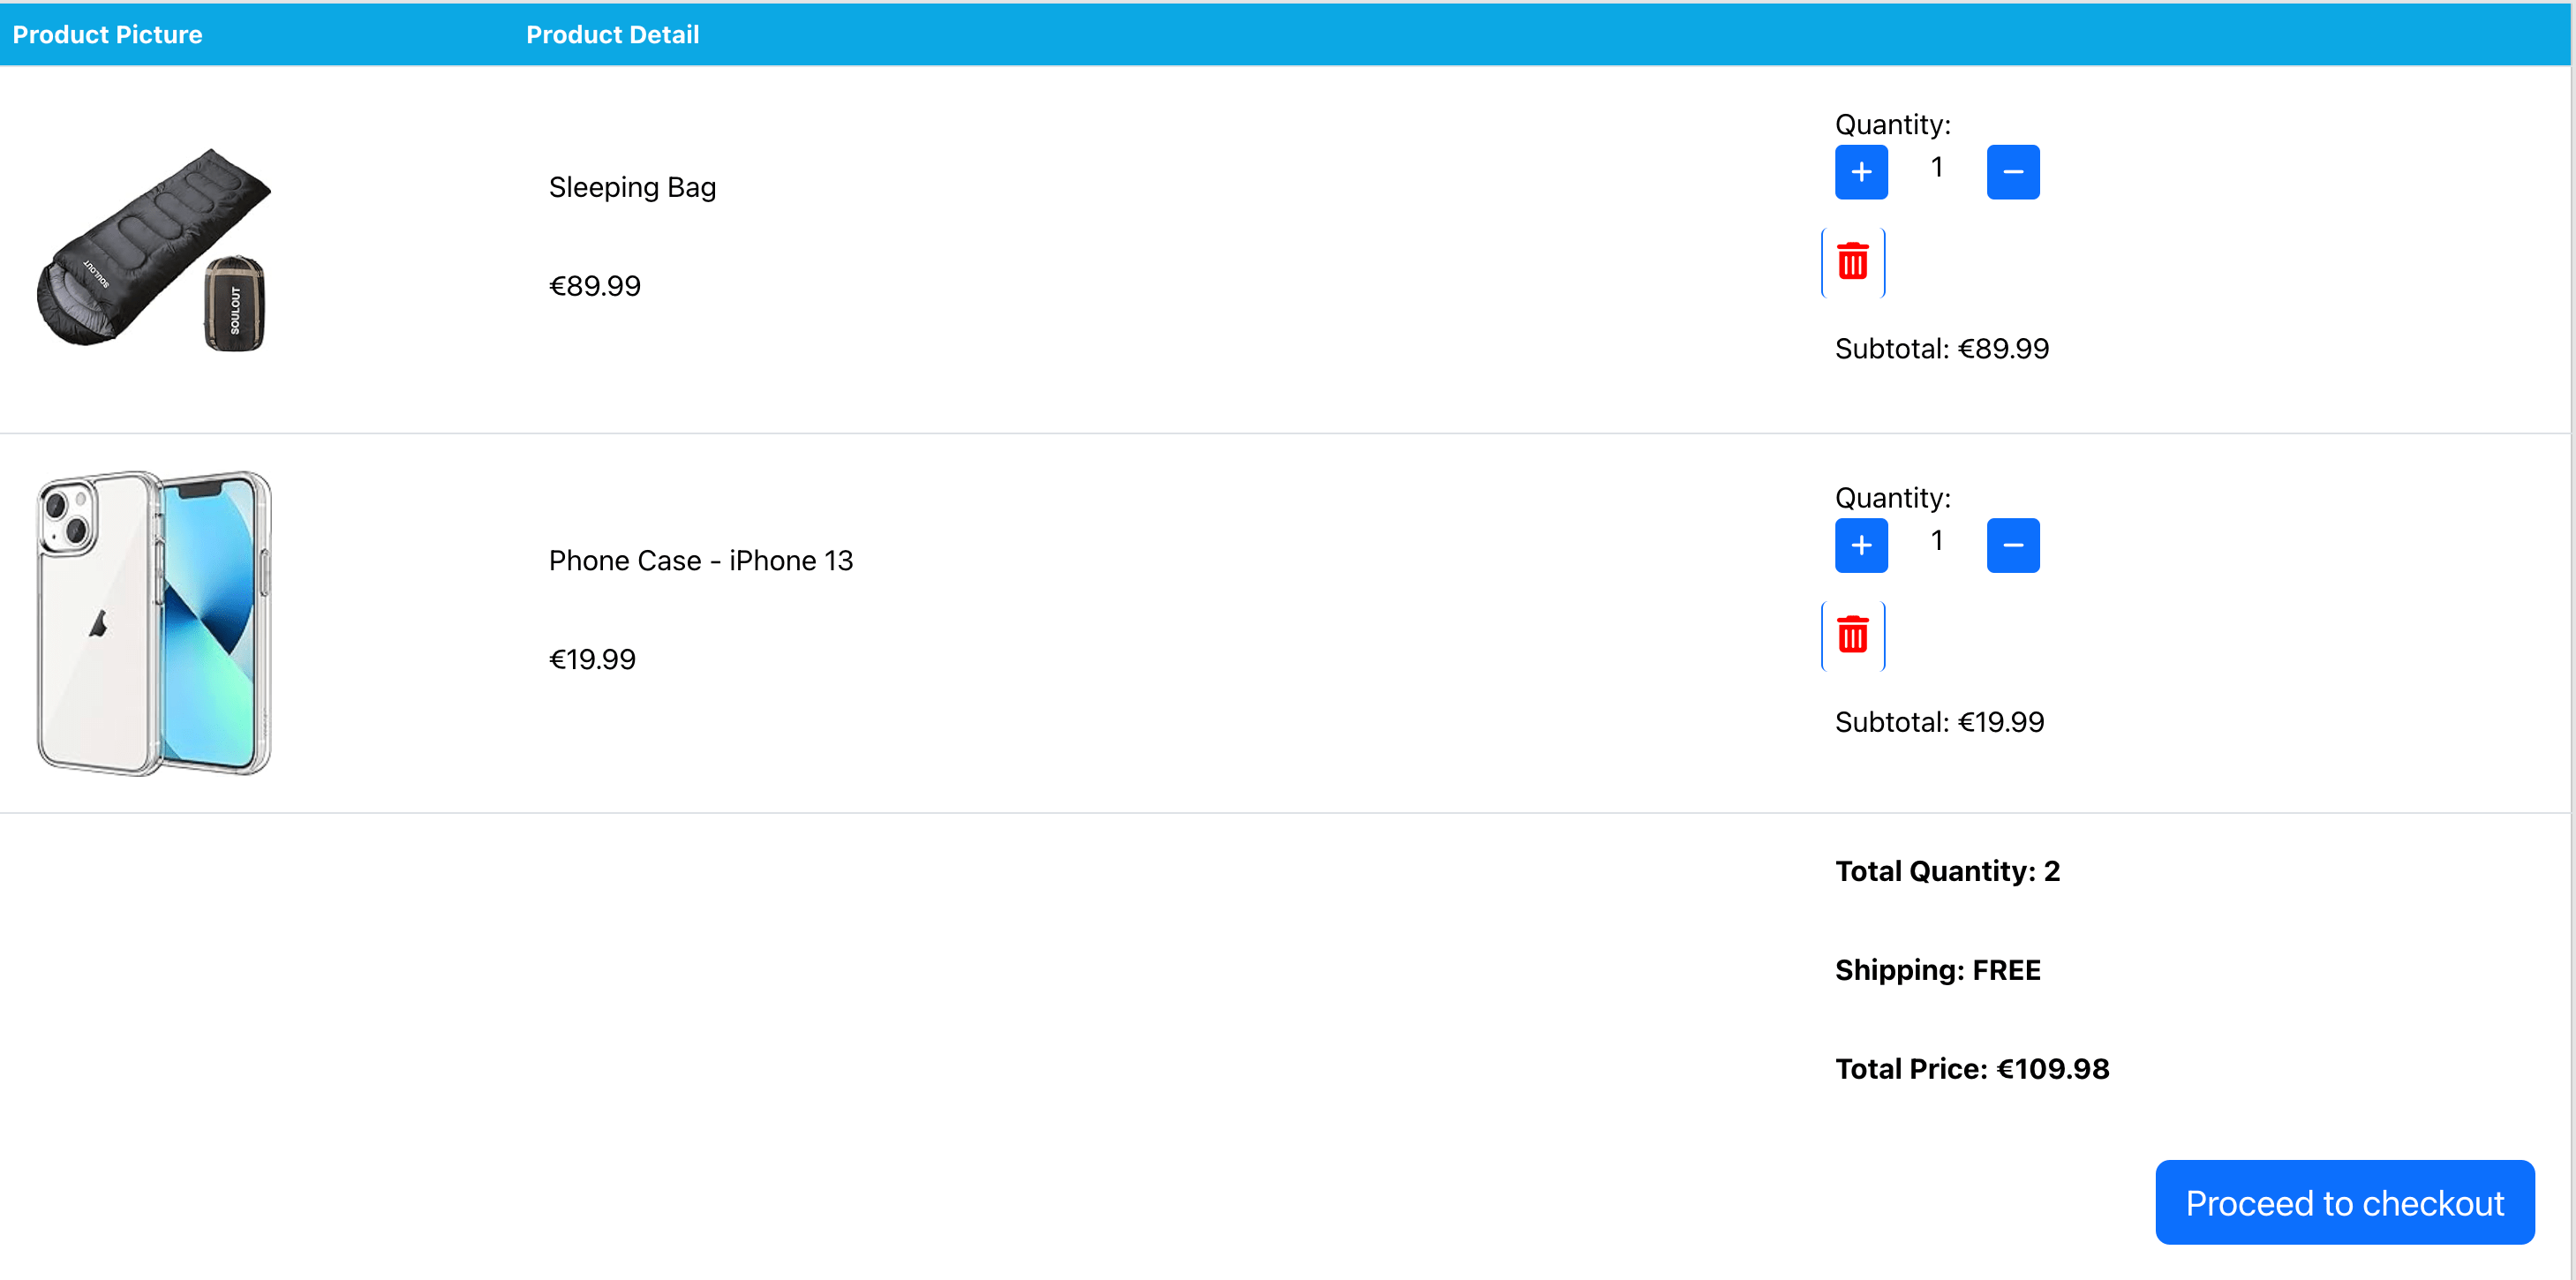
\includegraphics[width=0.9\textwidth]{Images/Cart-Details.png} 
	\caption{Warenkorb-Details} 
	\label{fig:sample2-image} 
\end{figure}

Die Detailseite des Warenkorbs bietet eine umfassende und benutzerfreundliche Schnittstelle, die mehrere Schlüsselelemente für ein optimales Einkaufserlebnis enthält. In der Produktliste werden alle Artikel angezeigt, die in den Warenkorb gelegt wurden, jeweils mit einem Bild und detaillierten Informationen. Der Benutzer kann seinen Warenkorb mit der Mengenkontrolle leicht verwalten, indem er die Menge jedes Produkts über Schaltflächen zum Erhöhen und Verringern anpasst oder Artikel nach Bedarf entfernt. Die Produktpreise werden übersichtlich dargestellt, einschließlich des Preises pro Einheit und der Zwischensummen, die auf der Grundlage der ausgewählten Menge berechnet werden. Die Bestellübersicht bietet einen Überblick über die Gesamtmenge der Artikel, wobei die Versandkosten als kostenlos gekennzeichnet sind und der endgültige Gesamtpreis deutlich angezeigt wird. Zur Erleichterung der nächsten Schritte im Kaufprozess ist eine auffällige Schaltfläche „Zur Kasse gehen“ enthalten, die den Benutzer zum Fortfahren mit der Bestellung anleitet.


\section{Checkout-Seite}\index{Checkout-Seite}
Nach einem Klick auf die Schaltfläche „Zur Kasse gehen“ leitet die Anwendung den Kunden zur Kassenseite weiter. Auf dieser Seite werden die Benutzer aufgefordert, ihre persönlichen Daten einzugeben, um den Kauf abzuschließen. Dazu gehören wichtige Angaben wie Name, Adresse und Zahlungsinformationen. Die Kassenseite ist so gestaltet, dass sie einen reibungslosen und sicheren Transaktionsprozess gewährleistet und den Benutzer durch die letzten Schritte zur Bestätigung seiner Bestellung und zum Abschluss des Kaufs führt.

Der erste Teil der Checkout-Seite (siehe Abbildung \ref{fig:sample3-image}) enthält ein Kundeninformationsformular, in dem die für die Auftragsabwicklung erforderlichen Angaben erfasst werden. Das Formular enthält Felder für grundlegende persönliche Informationen wie z. B.:

\begin{itemize}
	\item \textbf{Name:} Zur Identifizierung des Kunden.
	\item \textbf{Telefonnummer:} Für Kontaktzwecke.
	\item \textbf{E-Mail:} Für Auftragsbestätigungen und Aktualisierungen.
\end{itemize}

Darüber hinaus werden in dem Formular Informationen zur Lieferadresse erfasst:

\begin{itemize}
	\item \textbf{Land:} Zur Bestimmung der Versandregion.
	\item \textbf{Straße:} Die spezifische Lieferadresse.
	\item \textbf{Stadt:} Die Stadt für die genaue Zustellung.
	\item \textbf{Bundesland:} Das Bundesland oder die Provinz.
	\item \textbf{Postleitzahl:} Zur genauen Identifizierung des Standorts.
\end{itemize}

\begin{figure}[H]  
	\centering % Centers the image
	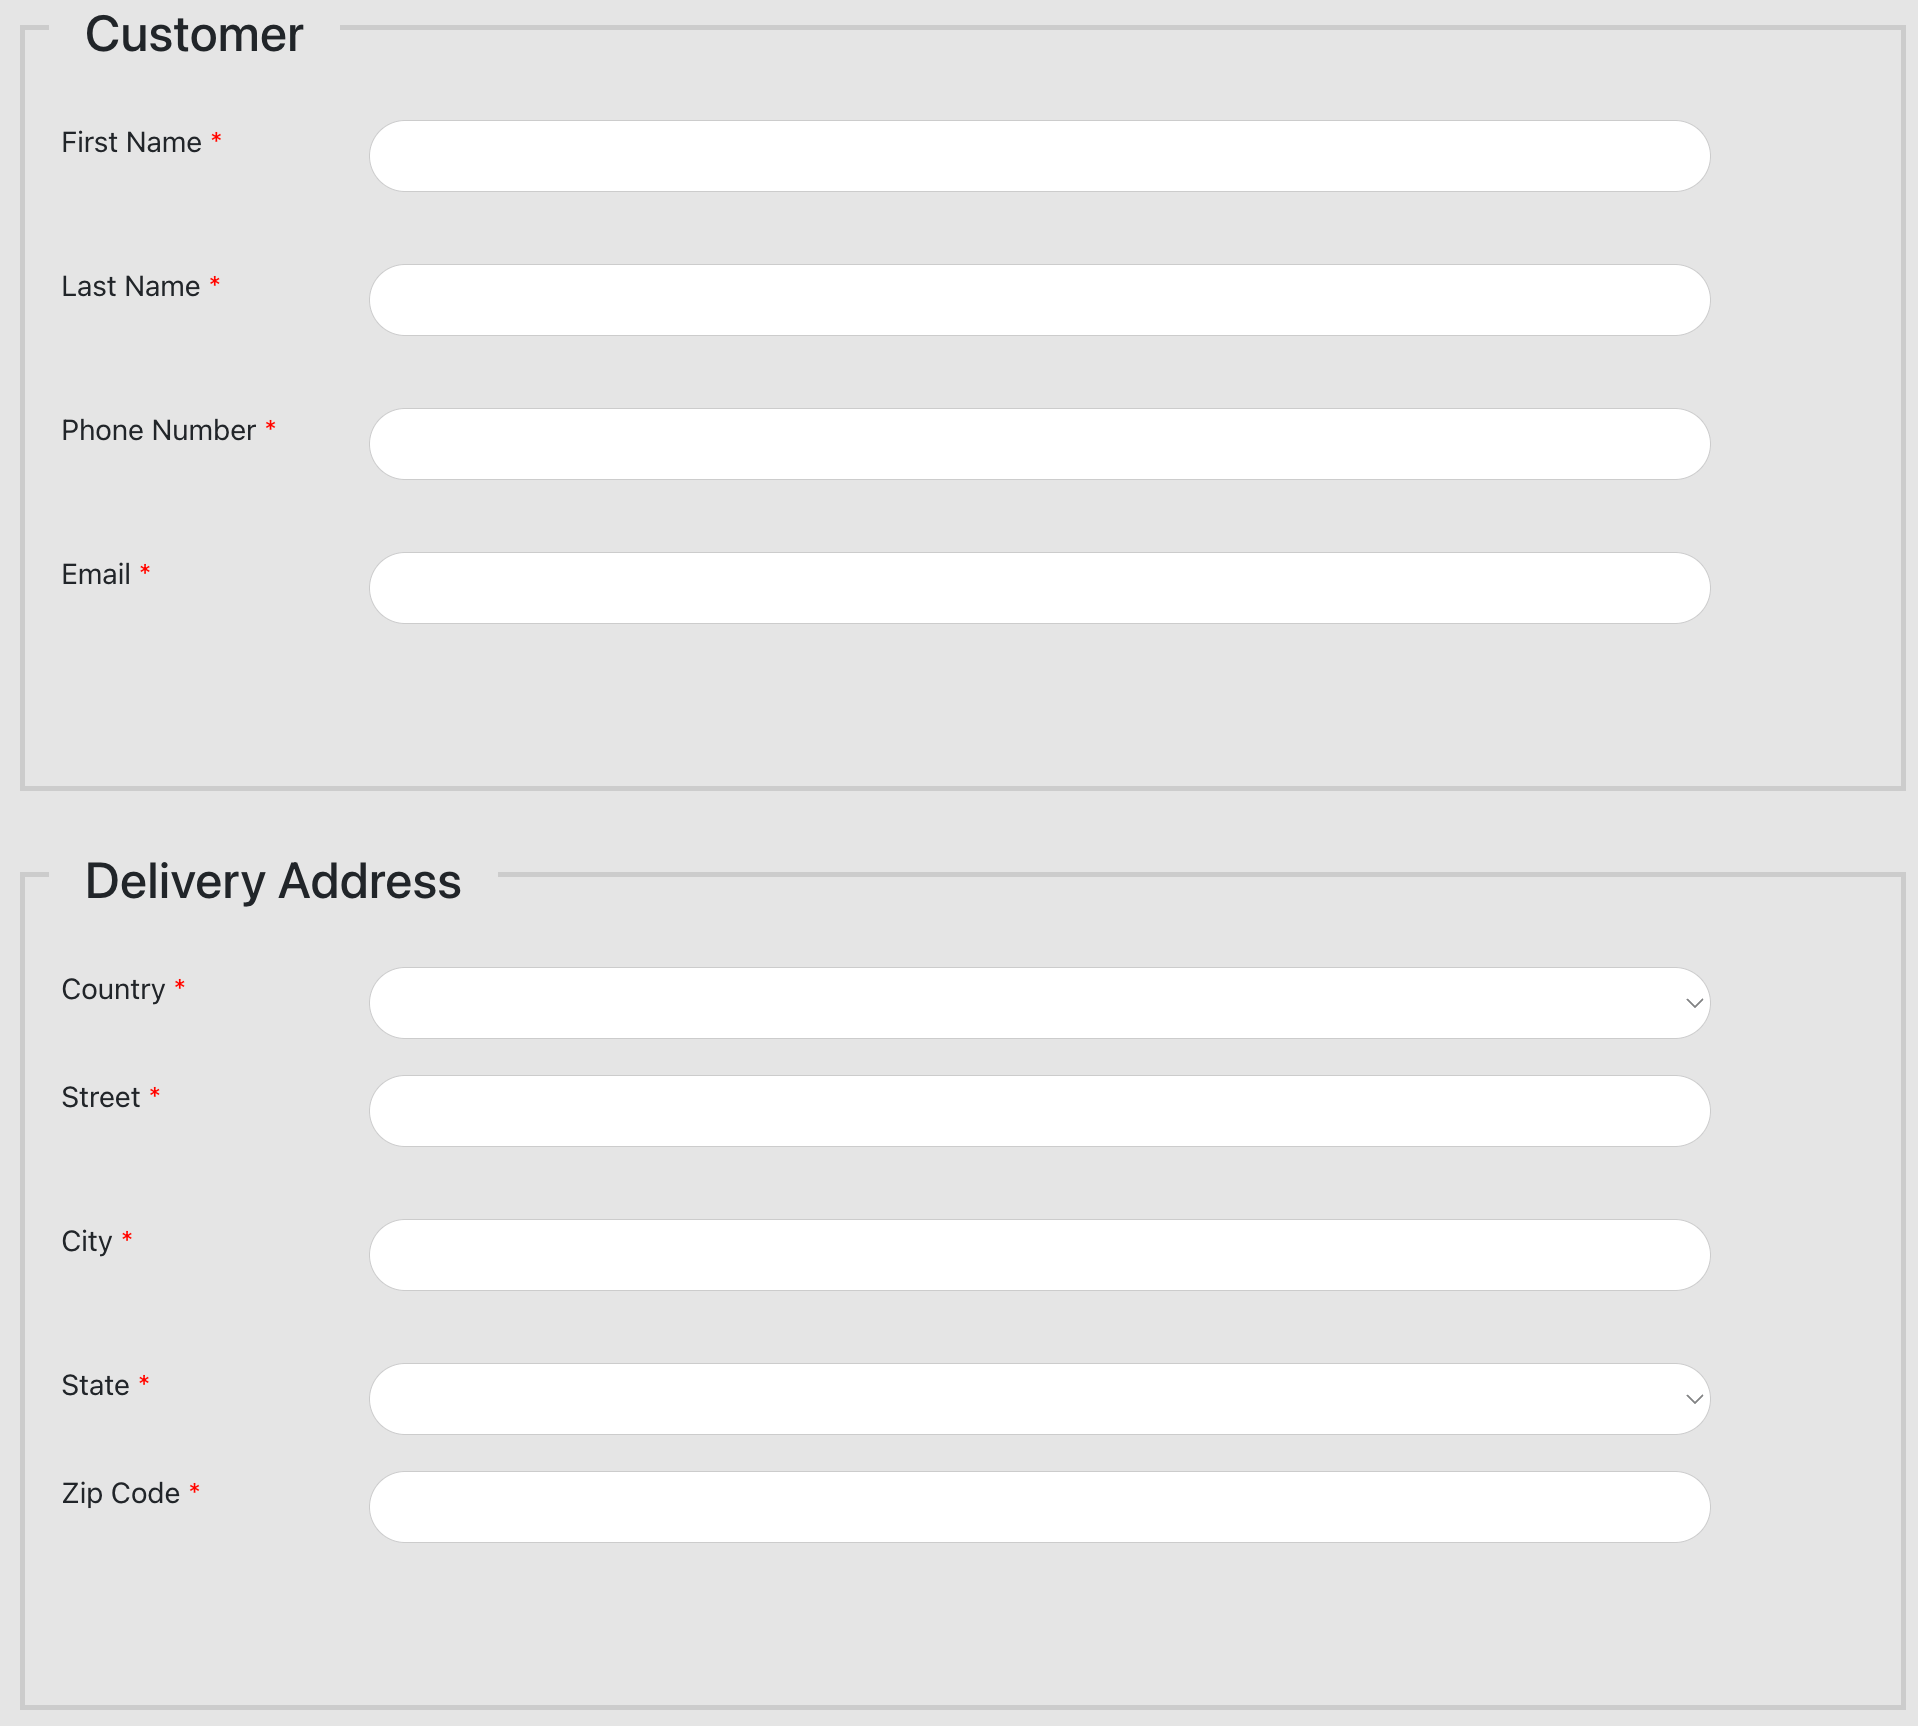
\includegraphics[width=0.9\textwidth]{Images/Checkout_1.png} 
	\caption{Checkout-1} 
	\label{fig:sample3-image} 
\end{figure}

Der Rest des Checkout-Formulars, wie in Abbildung \ref{fig:sample4-image} gezeigt, besteht aus:
\begin{itemize}
	\item Zahlungsadresse: Dieselbe wie die Lieferadresse.
	\item Zahlungsmethode: Akzeptiert Debit- oder Kreditkarten; erfordert Kartennummer, Gültigkeitsdatum und CVC-Code.
	\item Bestellübersicht: Zeigt die Gesamtzahl der Artikel, die Versandkosten und den Gesamtpreis an.
	\item Schaltfläche Kaufen: Ermöglicht es dem Benutzer, seinen Einkauf abzuschließen.
\end{itemize}

\begin{figure}[H]  
	\centering % Centers the image
	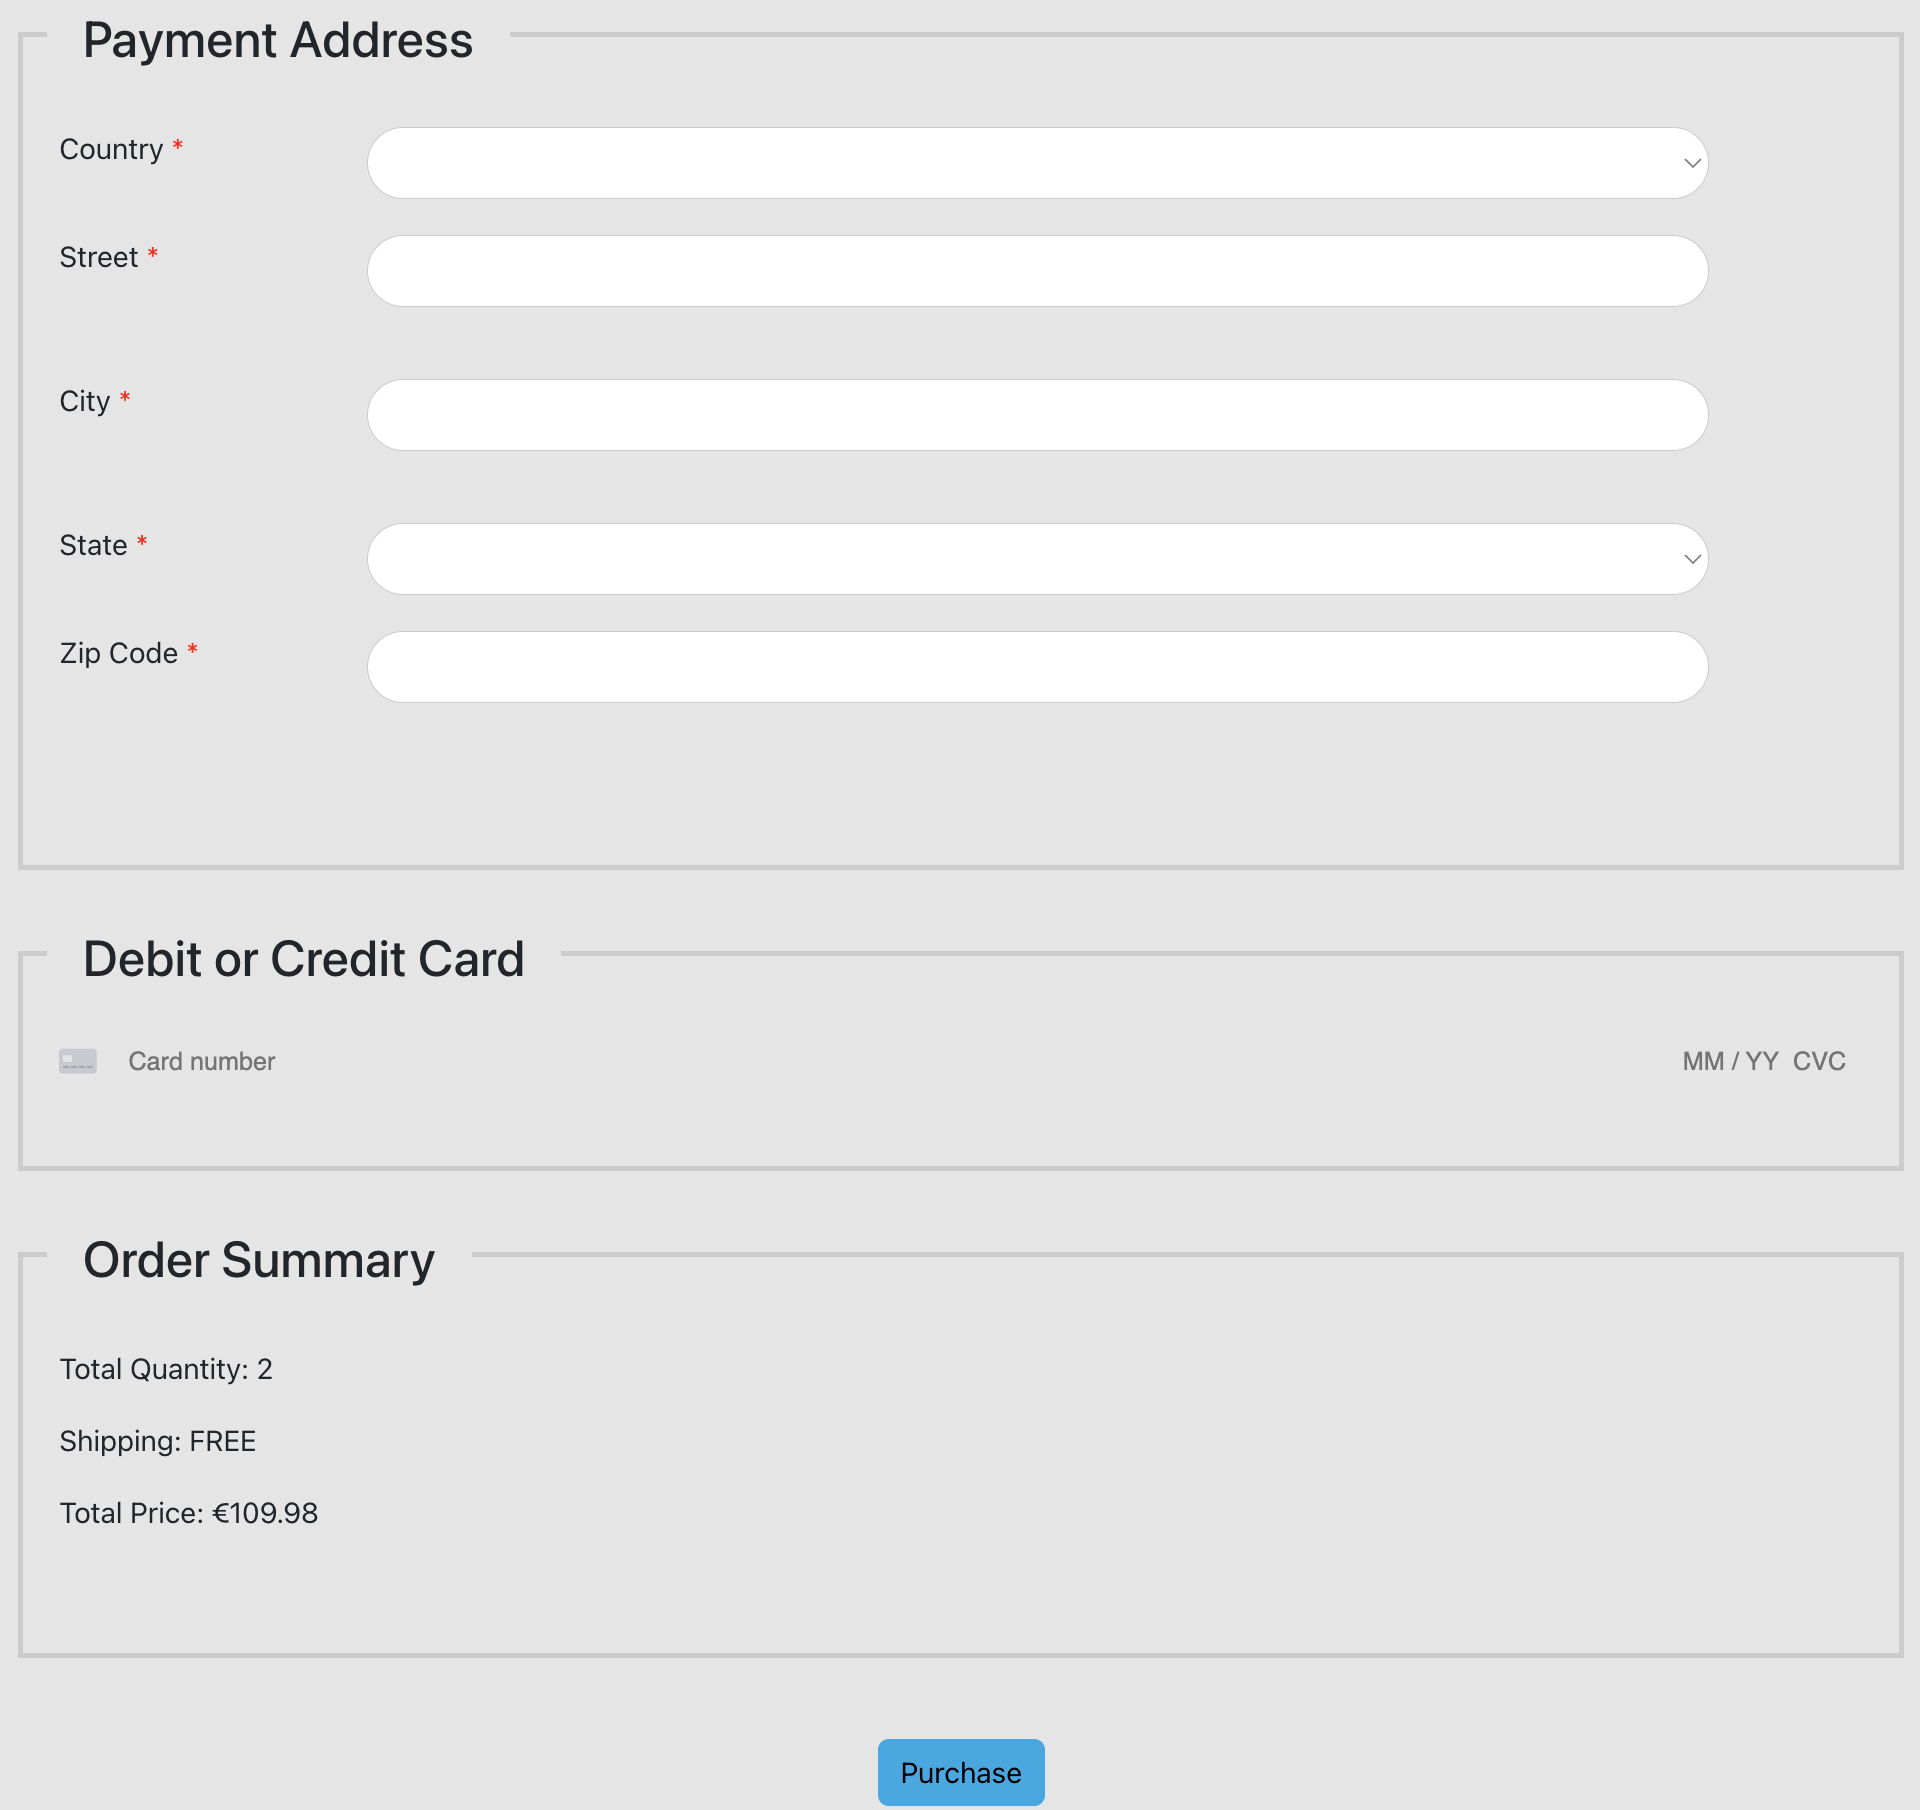
\includegraphics[width=0.9\textwidth]{Images/Checkout_2.png} 
	\caption{Checkout-2} 
	\label{fig:sample4-image} 
\end{figure}

Nach dem Klicken auf die Schaltfläche „Kaufen“ wird eine Benachrichtigung von localhost:4200 ausgelöst, die bestätigt, dass die Bestellung eingegangen ist (siehe Abbildung \ref{fig:sample5-image}). Die Nachricht enthält eine Referenznummer zur Auftragsverfolgung. Nach dieser Bestätigung wird der Kunde zur Homepage zurückgeleitet, und der Warenkorb wird geleert.

\begin{figure}[H]  
	\centering % Centers the image
	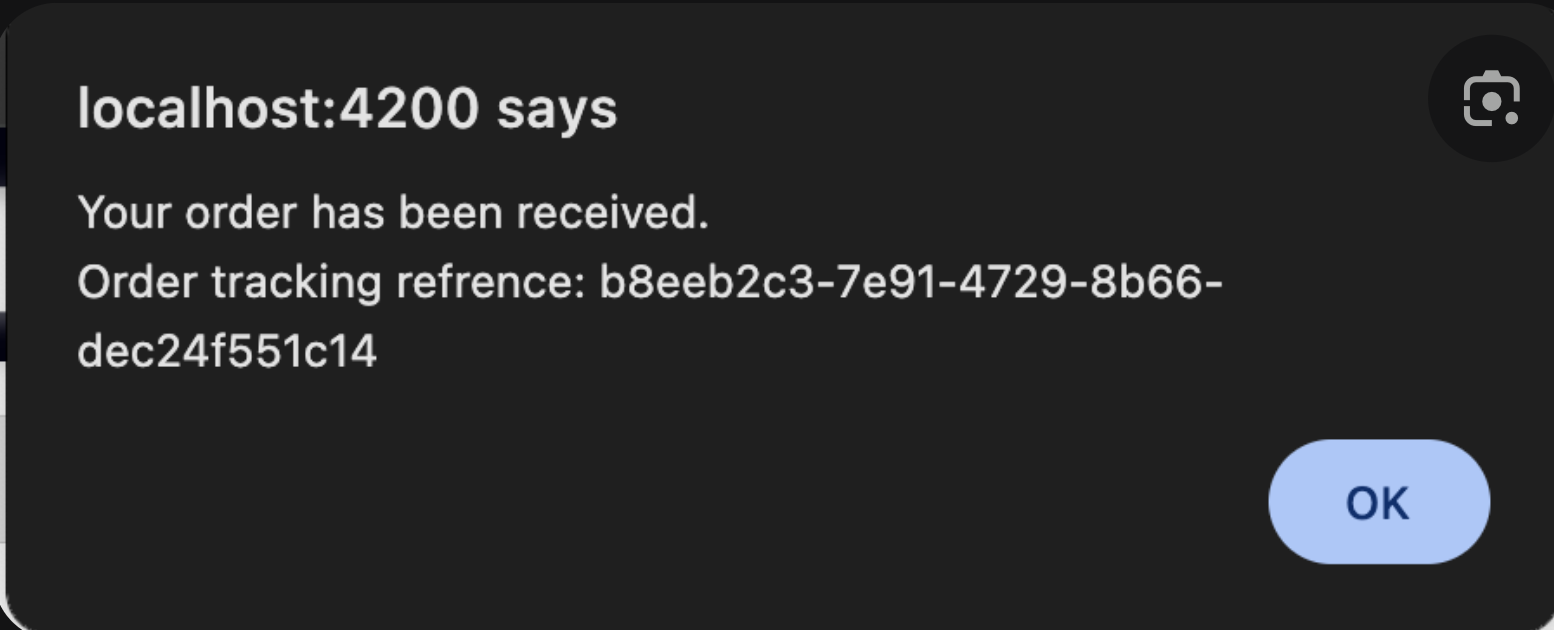
\includegraphics[width=0.9\textwidth]{Images/Purchase.png} 
	\caption{Purchase-Button} 
	\label{fig:sample5-image} 
\end{figure}

\section{Login}\index{Login}

Wie auf der Startseite zu sehen ist, gibt es eine Leiste mit einer Login-Schaltfläche, mit der sich Kunden authentifizieren können, um auf Seiten zuzugreifen, die nur für Mitglieder zugänglich sind. Die untenstehende Abbildung  \ref{fig:sample6-image} zeigt die Schnittstelle, die nach dem Klicken auf die Schaltfläche „Login“ erscheint.

\begin{figure}[H]  
	\centering % Centers the image
	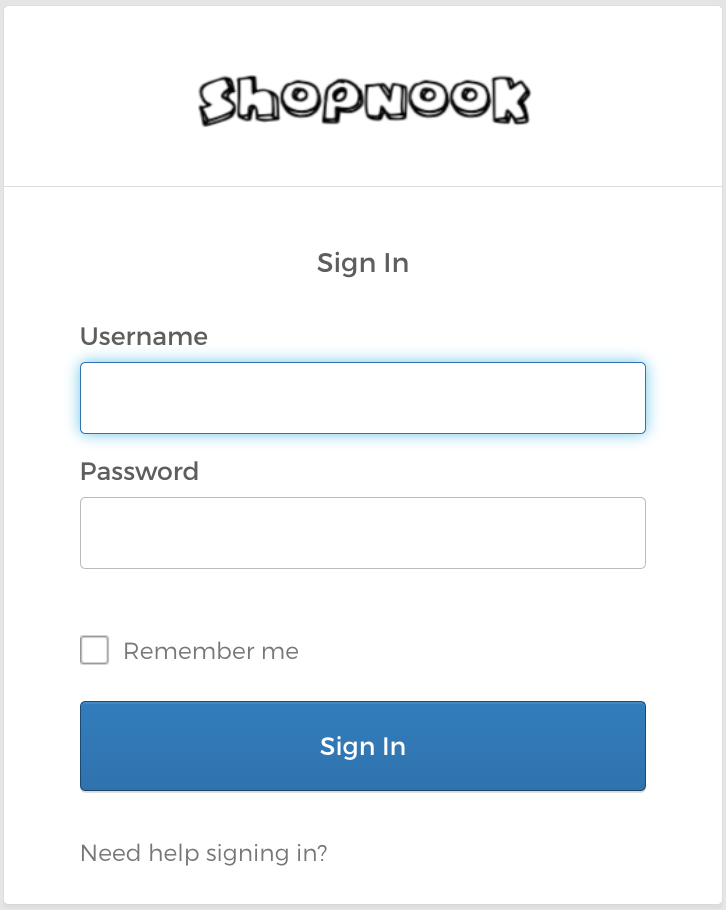
\includegraphics[width=0.6\textwidth]{Images/Login.png} 
	\caption{Login} 
	\label{fig:sample6-image} 
\end{figure}


Nach Eingabe der korrekten E-Mail und des Passworts leitet die App den Kunden zur Homepage weiter. Wie unten dargestellt (siehe Abbildung \ref{fig:sample7-image}), sieht der Kunde zwei Links, die nur eingeloggten Benutzern zur Verfügung stehen: Bestellungen, Mitgliederseiten und eine Schaltfläche „Logout“ zum Ausloggen.



\begin{figure}[H]  
	\centering % Centers the image
	
\includegraphics[width=0.9\textwidth]{Images/Login-bar.png} 
	\caption{Login-Leiste} 
	\label{fig:sample7-image} 
\end{figure}

 \subsection{Auftragsverlauf}

Nach dem Klicken auf „Orders“ zeigt das Bild eine Liste der letzten Bestellungen mit Details wie Bestellungsreferenz, Gesamtpreis, Gesamtmenge und Datum, wie unten (siehe Abbildung \ref{fig:sample8-image}) gezeigt.


\begin{figure}[H]  
	\centering % Centers the image
	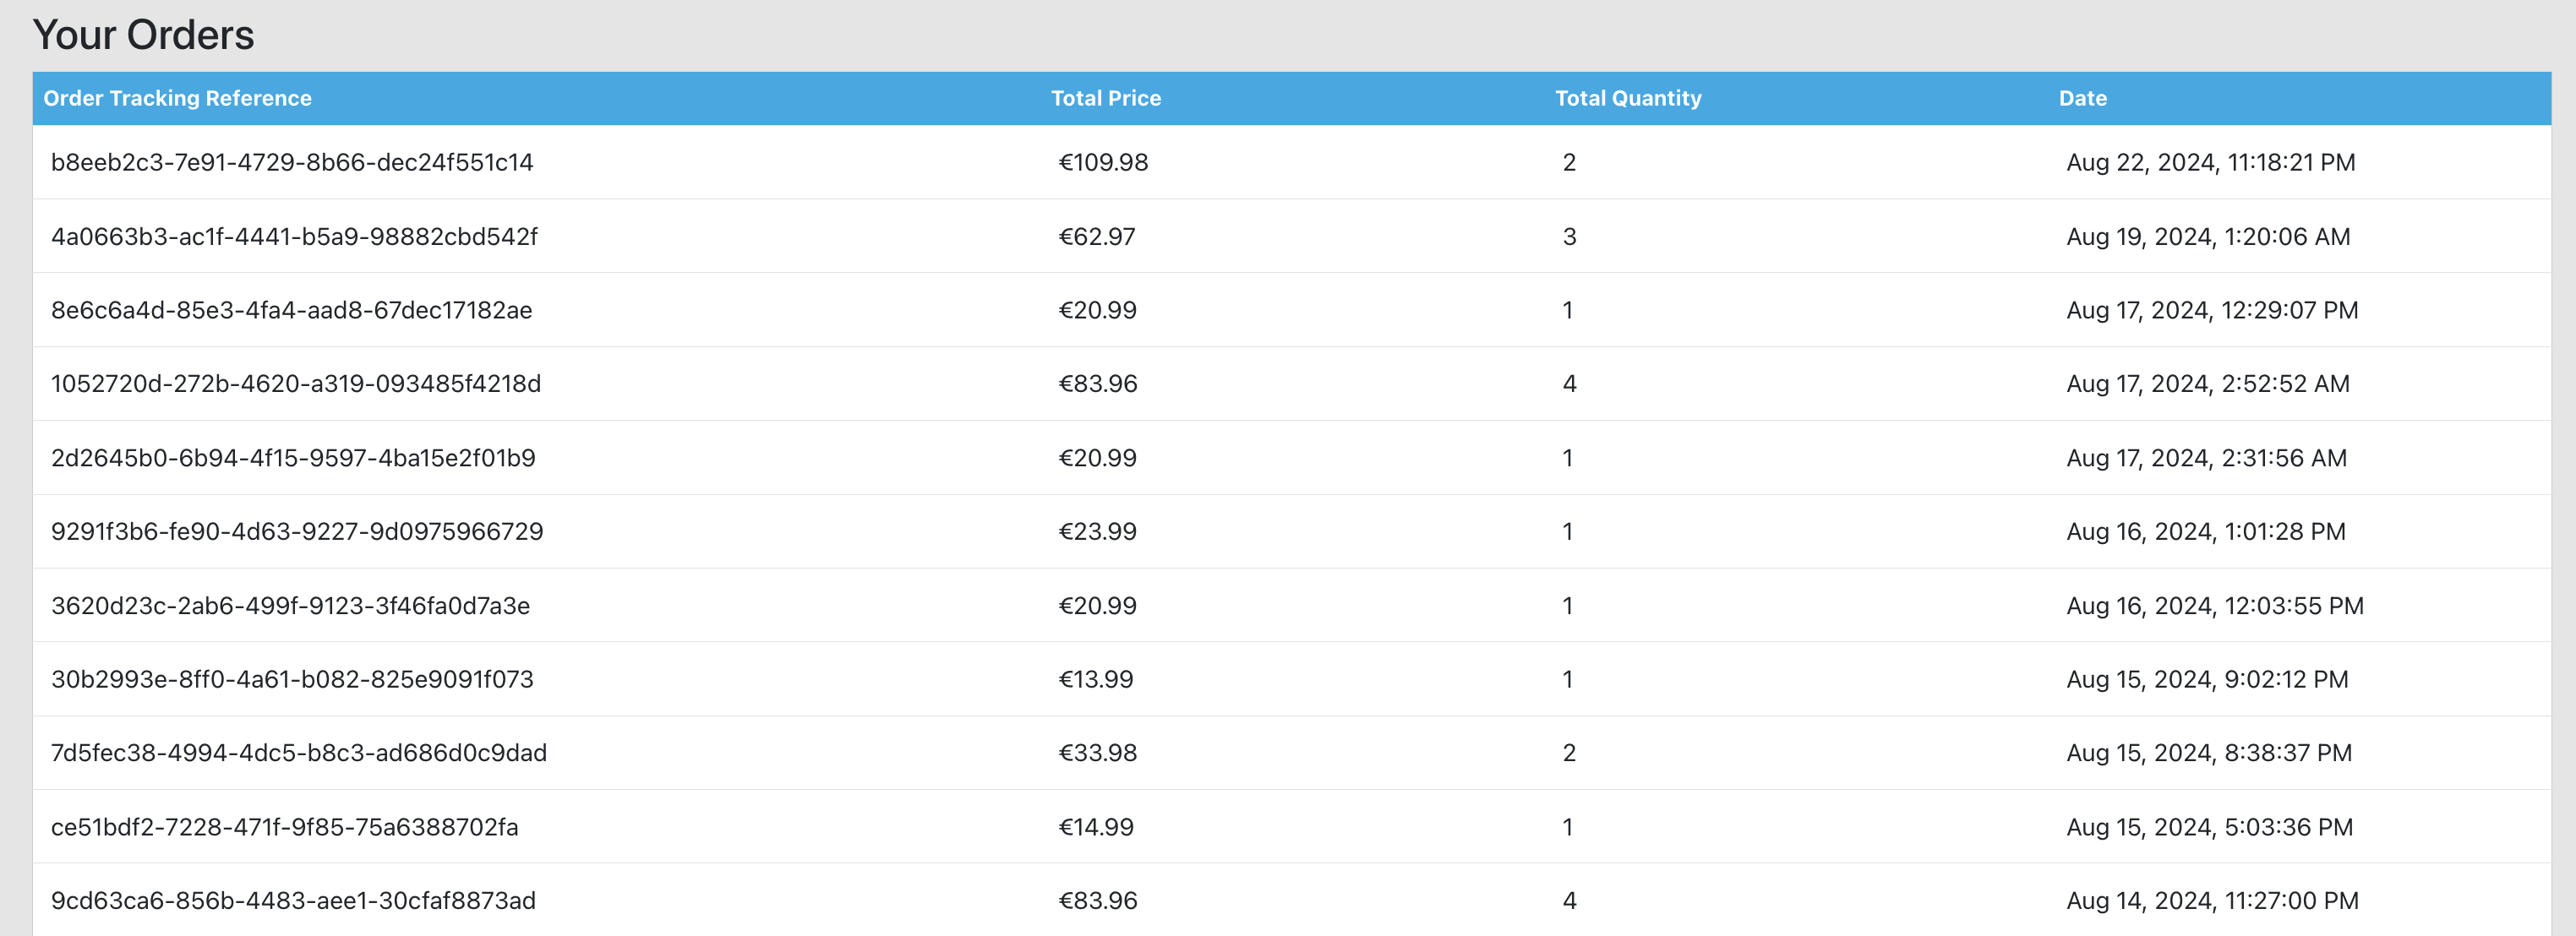
\includegraphics[width=0.9\textwidth]{Images/Orders-History.png} 
	\caption{Auftragsverlauf} 
	\label{fig:sample8-image} 
\end{figure}

 \subsection{Mitgliederseite}

Die Mitgliederseite bietet eine Vielzahl von exklusiven Inhalten, die auf angemeldete Benutzer zugeschnitten sind. Sie enthält aktuelle Angebote und Rabatte, die besondere Einsparungen bei ausgewählten Artikeln ermöglichen. Außerdem werden auf der Seite Produktempfehlungen angezeigt, die auf den Vorlieben und dem Surfverhalten der Nutzer basieren. Um das Einkaufserlebnis zu verbessern, werden auch Rückmeldungen anderer Kunden angezeigt, die Aufschluss über die Produktqualität und -zufriedenheit geben. Diese Kombination aus personalisierten Empfehlungen, Werbeaktionen und Erfahrungsberichten hilft den Mitgliedern, fundierte Kaufentscheidungen zu treffen und sich über die neuesten Angebote und Produkte zu informieren.\\

\noindent{Unten (siehe Abbildung \ref{fig:sample9-image})ist eine Illustration des Inhalts der Seite:} 

\begin{figure}[H]  
	\centering % Centers the image
	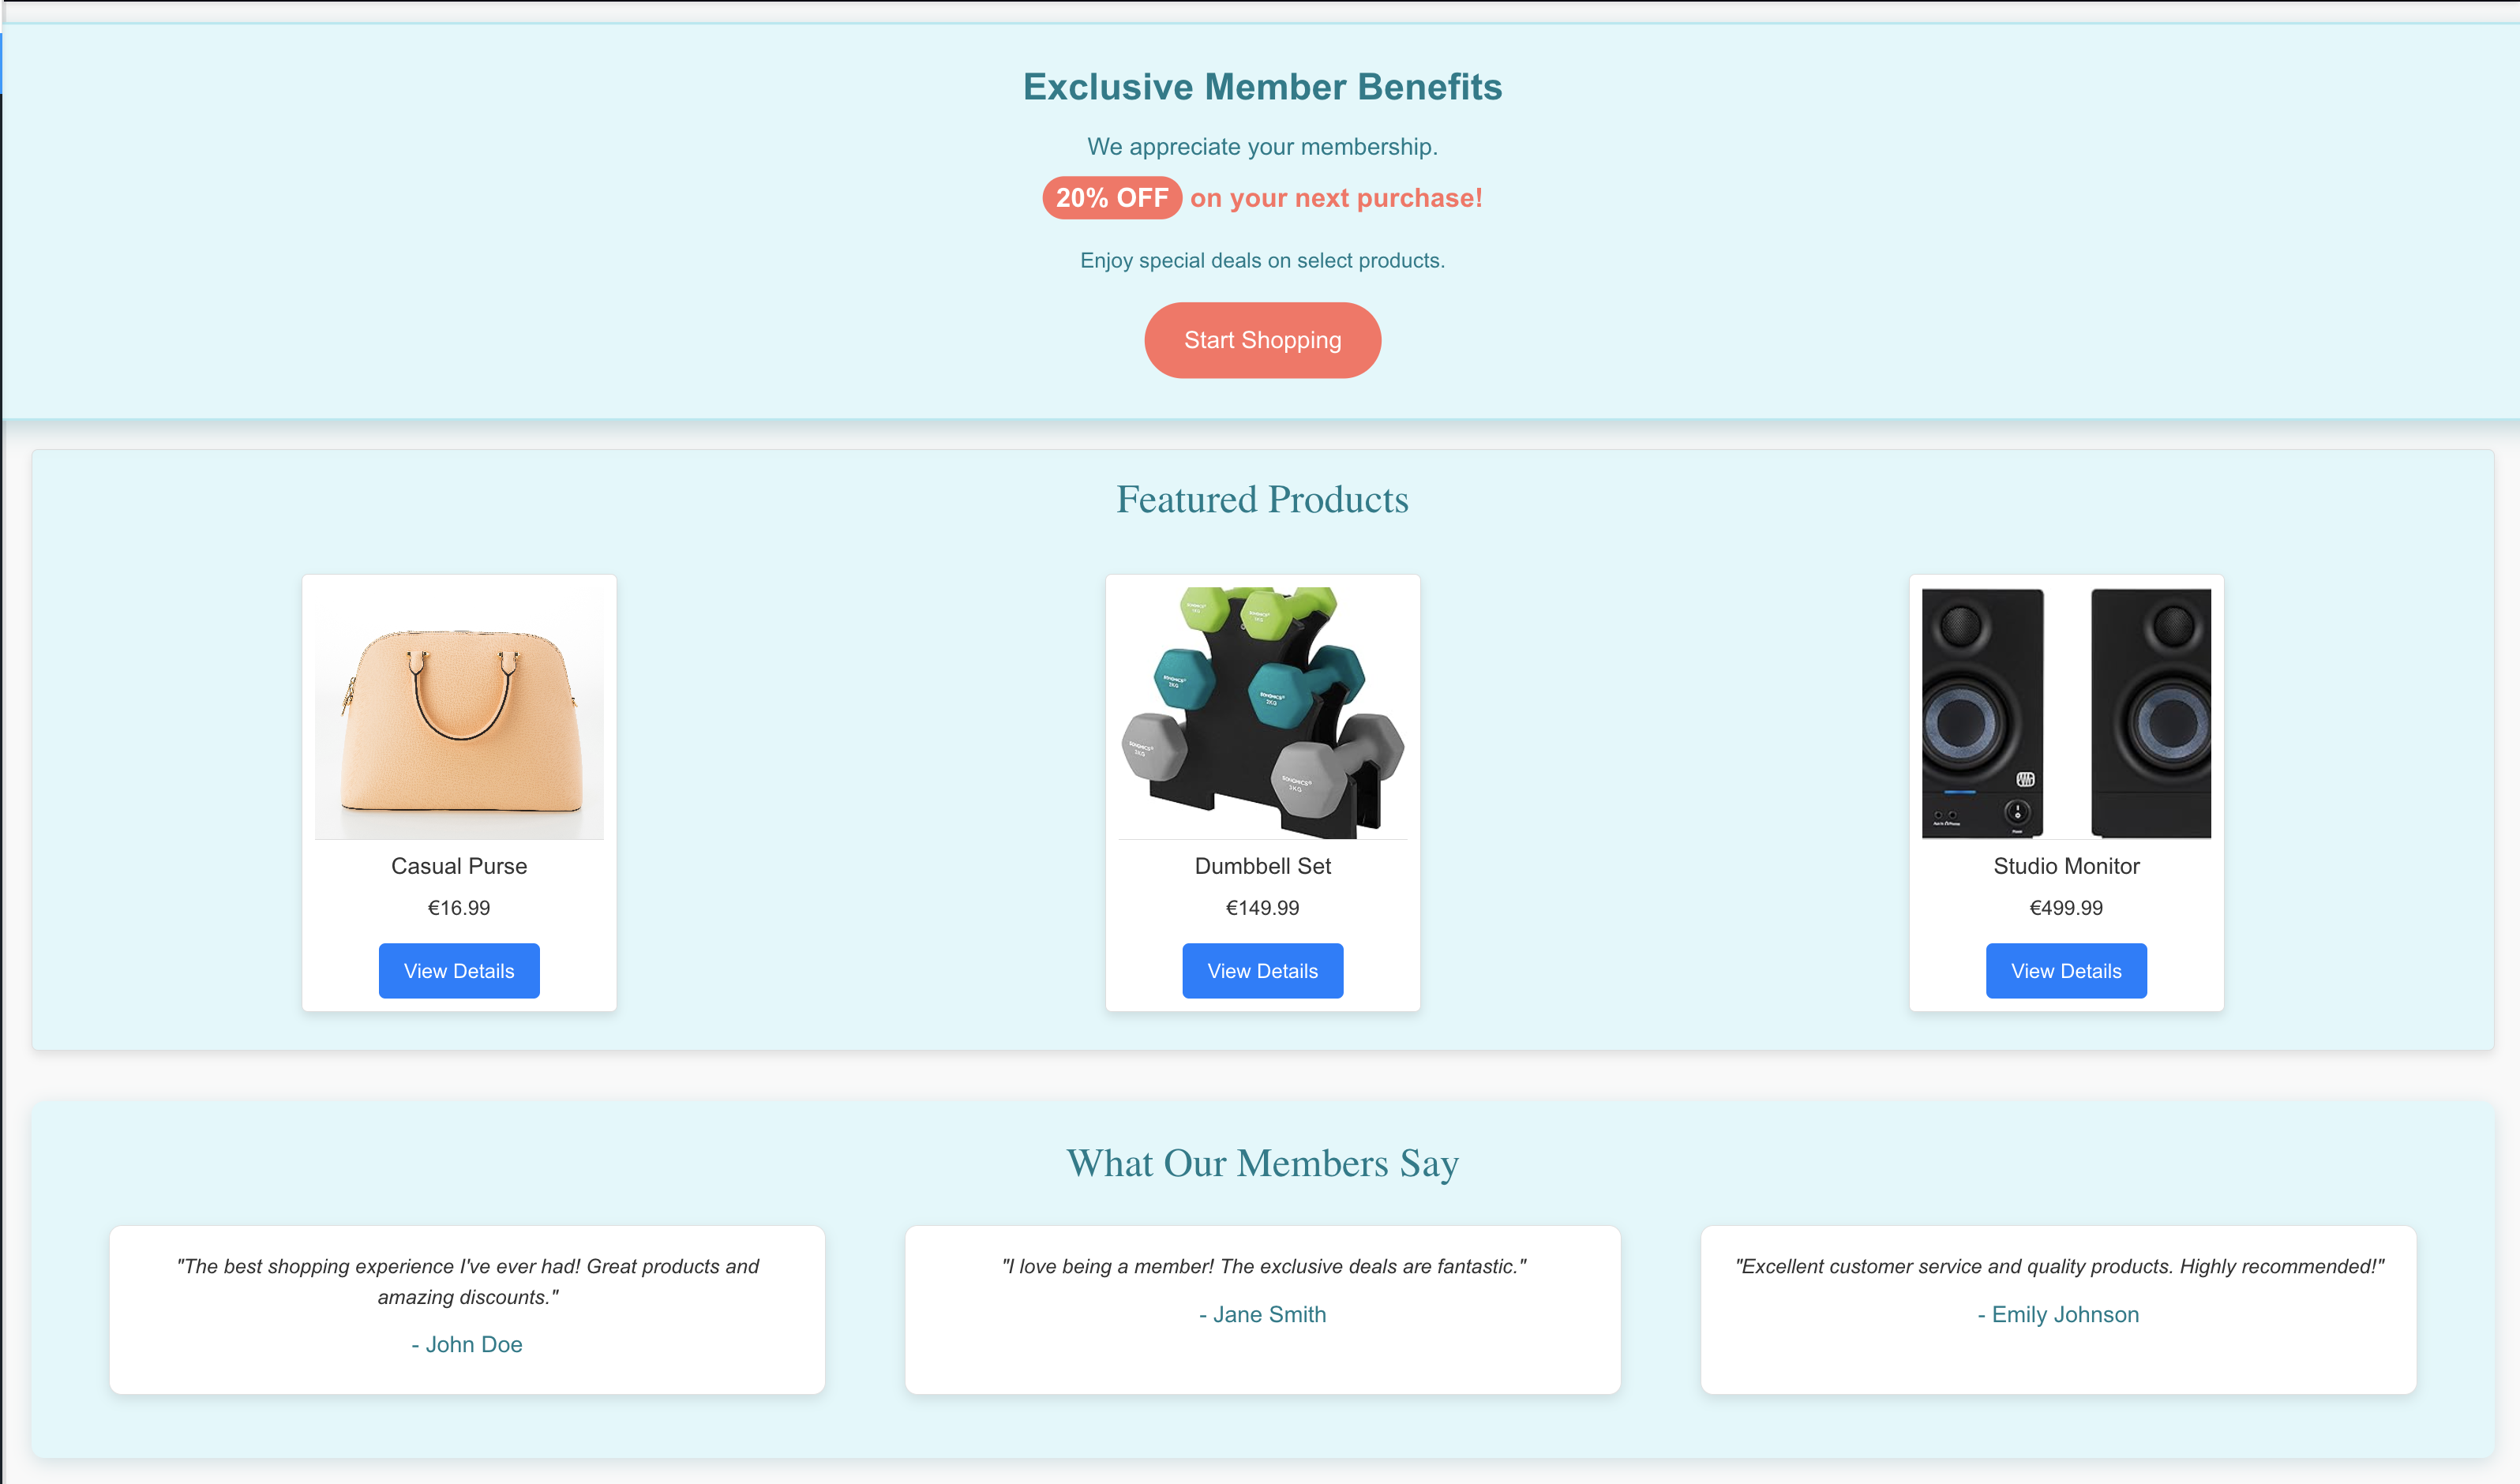
\includegraphics[width=0.9\textwidth]{Images/Member.png} 
	\caption{Mitgliederseite} 
	\label{fig:sample9-image} 
\end{figure}

\noindent{Abschließend werden anhand dieser Beispiele einige der wichtigsten Funktionen der E-Commerce-Web-App „ShopNook“ vorgestellt. Sie veranschaulichen die Kernaspekte der Benutzererfahrung und konzentrieren sich auf die Funktionalität und die Navigation innerhalb der Plattform.}






























\chapter{Zusammenfassung und Ausblick}

Im Rahmen dieser Arbeit werden mehrere Schwierigkeiten und Herausforderungen bei der Konzeptentwicklung und Umsetzung der E-Commerce-Warenkorbanwendung „ShopNook'' thematisiert. Zu den Herausforderungen gehören:

\begin{itemize}
	\item \textbf{Technische Integration}: Die nahtlose Integration der verschiedenen Technologien (Angular für das Frontend, Spring Boot für das Backend und MySQL für die Datenbank) stellte eine Herausforderung dar, insbesondere in Bezug auf die Kommunikation zwischen den Komponenten und die Sicherstellung der Datenkonsistenz.
	\item \textbf{Sicherheitsaspekte}: Die Implementierung von Sicherheitsmaßnahmen wie HTTPS-Verschlüsselung und JWT-basierte Authentifizierung erforderte sorgfältige Planung und Tests, um sicherzustellen, dass die Benutzerdaten und Transaktionen geschützt sind.
	\item \textbf{Benutzererfahrung}: Die Gestaltung einer intuitiven und ansprechenden Benutzeroberfläche, die auf verschiedenen Geräten gut funktioniert, war eine weitere Herausforderung. Es war wichtig, ein Gleichgewicht zwischen Funktionalität und Benutzerfreundlichkeit zu finden.
\end{itemize}

Allerdings sind offene Punkte geblieben, die noch weiter untersucht werden müssen, und sie umfassen:

\begin{itemize}
	\item \textbf{Leistungsoptimierung}: Es gilt herauszufinden, wie die Anwendung unter hoher Last performt und welche Maßnahmen zur Optimierung der Ladezeiten und der Reaktionsfähigkeit ergriffen werden können.
	\item \textbf{Erweiterte Funktionen}: Die Implementierung zusätzlicher Funktionen, wie z.B. personalisierte Empfehlungen oder ein verbessertes Bestandsmanagement, könnte die Benutzererfahrung weiter verbessern.
\end{itemize}



%------------------ Literaturverzeichnis & Index -------------------------------
\backmatter
\bibliography{literatur}								% Literaturverzeichnis (literatur.bib)
\printindex												% Index (optional)


%------------------ Anhänge ----------------------------------------------------
\begin{appendix}
	\chapter{Glossar}

\abbreviation{DisASTer}		{Distributed Algorithms Simulation Terrain, eine Plattform zur Implementierung verteilter Algorithmen \cite{Gottwald:03}}

\abbreviation{DSM}			{Distributed Shared Memory}

\abbreviation{AC}			{Atomic Consistency (dt.: Linearisierbarkeit)}
\abbreviation{RC}			{Release Consistency (dt.: Freigabekonsistenz)}
\abbreviation{SC}			{Sequential Consistency (dt.: Sequentielle Konsistenz)}
\abbreviation{WC}			{Weak Consistency (dt.: Schwache Konsistenz)}
							% Glossar (optional)
	\chapter{Selbstständigkeitserklärung}

\begin{description}


\item[$\Box$] Diese Arbeit wurde als Gruppenarbeit angefertigt. Meinen Anteil habe ich selbstständig verfasst und keine anderen als die angegebenen Quellen und Hilfsmittel verwendet.\\

Namen der Mitverfasser:
\vspace{3cm}


\begin{minipage}[t]{3cm}
	\rule{3cm}{0.5pt}
	Datum
\end{minipage}
\hfill
\begin{minipage}[t]{9cm}
	\rule{9cm}{0.5pt}
	Unterschrift der Kandidatin/des Kandidaten
\end{minipage}


\end{description}

\vspace{2cm}

\begin{minipage}[t]{3cm}
	\rule{3cm}{0.5pt}
	Datum
\end{minipage}
\hfill
\begin{minipage}[t]{9cm}
	\rule{9cm}{0.5pt}
	Unterschrift der Kandidatin/des Kandidaten
\end{minipage}
	% Selbstständigkeitserklärung
\end{appendix}


\end{document}
